%!TEX root = ../PhD_thesis__Lilian_Besson

% First chapter begins here
\chapter{Introduction}
\label{chapter:1}

% \abstractStartChapter{}%
% %
% We start by presenting the context then the problems studied in this thesis.
% We further announce the different directions we considered and the solutions we proposed.
% We give an overview of our main contributions, alongside a list of publications written in the last three years.
% %
% The organization of this manuscript is detailed in a flow graph, which highlights that Chapters~\ref{chapter:4} to \ref{chapter:6} are partly independent, but they are all built upon the model and notations introduced on Chapter~\ref{chapter:2}.

% \TODOL{J'enlève l'abstract et la minitoc dès que le chapitre est terminé !}

% \minitocStartChapter{}

% Write miniTOC just after the title
\graphicspath{{2-Chapters/1-Chapter/Images/}}

% Where
% \textbf{Where and when?}
%
This manuscript concludes my doctoral thesis, which started in October $2016$ and finished in November $2019$.
My research took place at the IETR laboratory in Rennes (France), in the SCEE team, hosted on the Rennes campus of the engineering school CentraleSupélec.
I was supervised by Professor Christophe Moy, in Rennes,
and I was also co-supervised by Doctor Émilie Kaufmann, whom I visited many times at Inria Lille Nord Europe in Lille (France).


% ----------------------------------------------------------------------------
\section{Context of this thesis}
\label{sec:1:problems}

% % Main problem
% \textbf{Main problems.}
%
The root of the problems motivating this thesis are the questions of global warming and the increase of the world population.
% https://en.wikipedia.org/wiki/History_of_radio
In the last $150$ years, humankind has developed different communication technologies, and since the late $1890$s, wireless communications between manufactured devices have been made possible, and more and more frequent in our lives.
With the advent of Internet of Things networks (IoT), billions of autonomous low-power devices are expected to be deployed worldwide, allowing a wide range of different applications.
It is now a world-wide consensus that with the current trend of population increase and with the ongoing energy crisis, any newly deployed technology should be both cheap and energy efficient,
as well as adapted to serve a large number of people and devices.
%
Such IoT technologies should be able to adapt automatically to different environments and application contexts, and be as efficient as possible.
%
In addition to the usual Research and Development effort to design different efficient radio access schemes, covering all the possible cases,
now the time has come to combine it with cheap and promising Machine Learning in order to (try to) attain the level of performance gain necessary for the IoT promises to become reality.

That is why we are interested in this thesis about
improving the battery life of IoT end-devices and reducing the energy cost of IoT networks.
We propose to attain these two goals jointly, by embedding low-cost decentralized decision making on directly into the future IoT devices.
%
Our focus in this PhD thesis is thus on the possible applications of embedding a certain kind of Machine Learning algorithms (Multi-Armed Bandit algorithms), in order to let the IoT devices optimize their wireless communications and learn to be self-organized automatically and without central control nor coordination.


\paragraph{From old TV to the IoT standards.}
%
Historically, three main families of wireless communication systems have been deployed in massive commercial networks: first, centralized broadcasting (\eg, radio or TV broadcasting), then centralized bi-directional systems (\eg, 4G or Wi-Fi), and nowadays decentralized data harvesting for the Internet of Things (IoT) networks (\eg, sensor networks).
%
% % Central broadcasting
% Starting from FM radio music and news, then old black-and-white TV and color TV, the first systems were purely made for centralized broadcasting of information. In a large area, one well located antenna emits continuously in a fixed Radio Frequency (RF) band, and many devices can listen to this RF signal and demodulate it, for instance to listen to some music.
% Different standards have been developed, and some of them are still in use today, and their nature requires a central authority that allocates RF bands to different usages (\eg, TV or FM radio channels etc).
% For example, in the city of Cesson-Sévigné where the campus of CentraleSupélec is located, a high RF tower emits on many standards, and in particular the \SI{92.3}{\mega\hertz} band is allocated to a French classical music radio (\emph{Radio Classique}).
% Broadcast-based systems are not only used for TV or radio:
% another famous and worldwide deployed example of mono-directional radio systems are the long-range global navigation satellite systems (such as USA's GPS or European Union's Galileo).
% %  and short-range infrared remote controllers.
% % https://en.wikipedia.org/wiki/Satellite_navigation
%
% % Two ways communications
% However, this kind of mono-directional wireless communications were soon found to not be satisfactory for many applications, and thus bi-directional standards were defined from the $1910$s.
% First developed by and for the military and the navy (\eg, the Titanic sent the first ``SOS'' signal over radio in $1912$),
% such applications have reached general public usage since the $1950$s.
% The greatest achievement of this long-running R\&D domain was the avent of mobile telephony in the $1990$s, which has continued to be more and more present in people's lives in all over the world, with the booming of personal cellphones since the $2000$s and smartphones since the $2010$s.
% In most systems, there is still a base station (with one or more antenna) in charge of a large area (or cell), and many devices are able to receive and transmit data to the base station.
% Nowadays, the most well-known systems include Wi-Fi, and systems deployed for mobile phone communications, with a long list of standards from 2G, 3G, 4G and now 5G, still in development in $2019$.
% Even if both systems initially differed in usage, as 2G was designed to exchange only voice, and Wi-Fi to link wireless devices at home to an Internet-connected box, they are conceptually very close.
% As the systems are cellular, any device knows the base station it is associated with, and the bi-directional nature of their exchanges makes a centralized control possible.
% In order to optimize the efficiency of the network, the base station is equipped with decision making algorithms that affects the devices in the cell to the available resources (time slots, RF bands, transmission power etc).
% To be able to communicate with the base station without interfering with each others, such affectation should be orthogonal, and led to systems based on Time (TDMA), Frequency (FDMA) and Code Division Multiple Access (CDMA).
% %  and Non-Orthogonal techniques only started to emerge recently (\eg, NOMA).
% Traditionally, the base station aimed only at maximizing the Quality of Service (QoS), that englobes the data rate, latency, availability and other measures of performance, of the wireless communications to and from the devices.
% More recently, ``green radio'' has emerged as a solution to the tradeoff between maximizing the QoS of the system, and minimizing the power consumption of the base station and the devices it serves.
%
%
% The opposite: decentralized broadcasting, and the age of IoT
% Finally, a third kind of systems are of the opposite kind,
This third kind of systems can be designed as decentralized:
because even if a central base station is still in charge of many devices,
the devices initiate the sending of up-link packets, and the only down-link data they can receive are short acknowledgements, sent from the base-station to indicate success or failure of every up-link packet.
This family of wireless systems are referred to as Internet of Things (IoT),
and a typical example of application of such IoT networks is for sensor wireless networks.

For the future development of ``smart grids'', ``smart cities'', ``smart homes'', or ``smart agriculture'', sensor networks are promised to be widely deployed.
Two examples of future applications that are already in deployment, in France or other countries, are ``connected buildings'' and ``connected agriculture''.
For buildings, the main goal is to reduce the cost of heating empty buildings and use sensor networks to get accurate and regular data about the temperature in all rooms and floors, and let the centralized heat control optimize its cost and energy consumption.
For agriculture, one example can be to equip every cow (in large farms) with sensors that regularly emit biological information, such as body temperature or stress level etc, in order to optimize the time of milking, to monitor the health of the animals etc.
%
% OK commencer par un paragraphe qui explique qu'on étudie les télécom dans le but de les rendre automatiquement plus efficace, plus verte, plus adaptative

This third kind of wireless systems is characterized by its decentralized nature,
where communications are initialized and regulated by the devices, not by a centralized control systems.
% due to the really limited information that the base station can send to the devices (in down-link), it is no longer possible to optimize the efficiency of the network from the centralized point-of-view of the base station.
Indeed, a central control requires signaling packets that have been identified as too heavy for these kinds of systems.
In the present and future IoT networks, many devices of heterogeneous natures are using the same antenna for different applications.
A common problem is the strong constraint that such IoT devices have on their power consumption, as most of them will be deployed without a direct power access and will run on a tiny battery, which lifespan should be maximized.
Most commercial IoT companies nowadays indeed sell a lifespan larger than $10$ years, like SIGFOX \cite{Centenaro16}.
Another common constraint for IoT devices is their low duty cycles, as most applications target a need for one or a few messages to send every day, in strike opposition to the high data-rate pursued for centralized systems (such as 4G/5G and Wi-Fi).
%
Many different standards for IoT networks have been proposed in the recent years,
and they consist in a specification for both the \emph{PHY}sical
and the \emph{M}edium \emph{A}ccess \emph{C}ontrol (\emph{MAC}) layers.
To quote some examples of IoT standards, ZigBee, Z-Wave or Bluetooth are targeting short-range communications (up-to \SI{2}{\meter}), while LoRaWAN, SIGFOX, Ingenu or Weightless are designed for long-range communications (up-to \SI{50}{\kilo\meter}).
We refer to the survey \cite{Centenaro16} and references in our recent articles \cite{MoyBesson2019,MoyBesson2019Annales} for more details.

% OK commencer par décrire ce sur quoi porte la thèse, en deux phrases qui réduisent le cadre


\paragraph{Spectrum Scarcity.}
%
A major problem of current wireless technologies is the issue of spectrum scarcity:
in most kinds of frequency bands, the entire RF spectrum is now allocated and free bands no longer exist, and this limits the possibility of adding any new usage.
As illustrated in Figure~\ref{fig:1:United_States_Frequency_Allocations_Chart_2016_The_Radio_Spectrum} below,
% only a very small portion of the RF spectrum in the USA is not yet allocated, from $0$ to \SI{9}{\kilo\hertz},
% while the rest of the displayed portion of the spectrum, from \SI{9}{\kilo\hertz} to \SI{300}{\giga\hertz},
almost the entire spectrum
is allocated to various usages, that goes from maritime radio-navigation (historically the first usage of radio telecommunication, \eg, in the Titanic), to space research, inter-satellite, mobile telephony and many other applications.
%
% Traditional regulatory structures have been built for an analog model and are not optimized for cognitive radio.
Regulatory bodies in the world, like the
\href{https://www.itu.int/en/Pages/default.aspx}{International Telecommunication Union} (see \href{https://www.itu.int/}{\texttt{www.ITU.int}}),
the \href{https://www.fcc.gov/}{Federal Communications Commission} in the United States of North America (see \href{https://www.fcc.gov/}{\texttt{FCC.gov}})
or the \href{https://cept.org}{European Conference of Postal and Telecommunications Administrations} in Europe (see \href{https://www.CEPT.org/}{\texttt{CEPT.org}}),
% or \href{http://www.tdf.fr/}{TDF} in France (see \href{https://www.TDF.fr/}{\texttt{TDF.fr}}),
as well as different independent measurement campaigns, found that most radio frequency spectrum are inefficiently utilized.
This means that while a band can be allocated to a certain unique usage, it can be free from any user in certain times and/or places.
We refer to \cite{patil2011survey} for a survey on the worldwide spectrum utilization, and to \cite{valenta2010survey} for the situation in Europe.


\begin{figure}[h!]
    \centering
    % 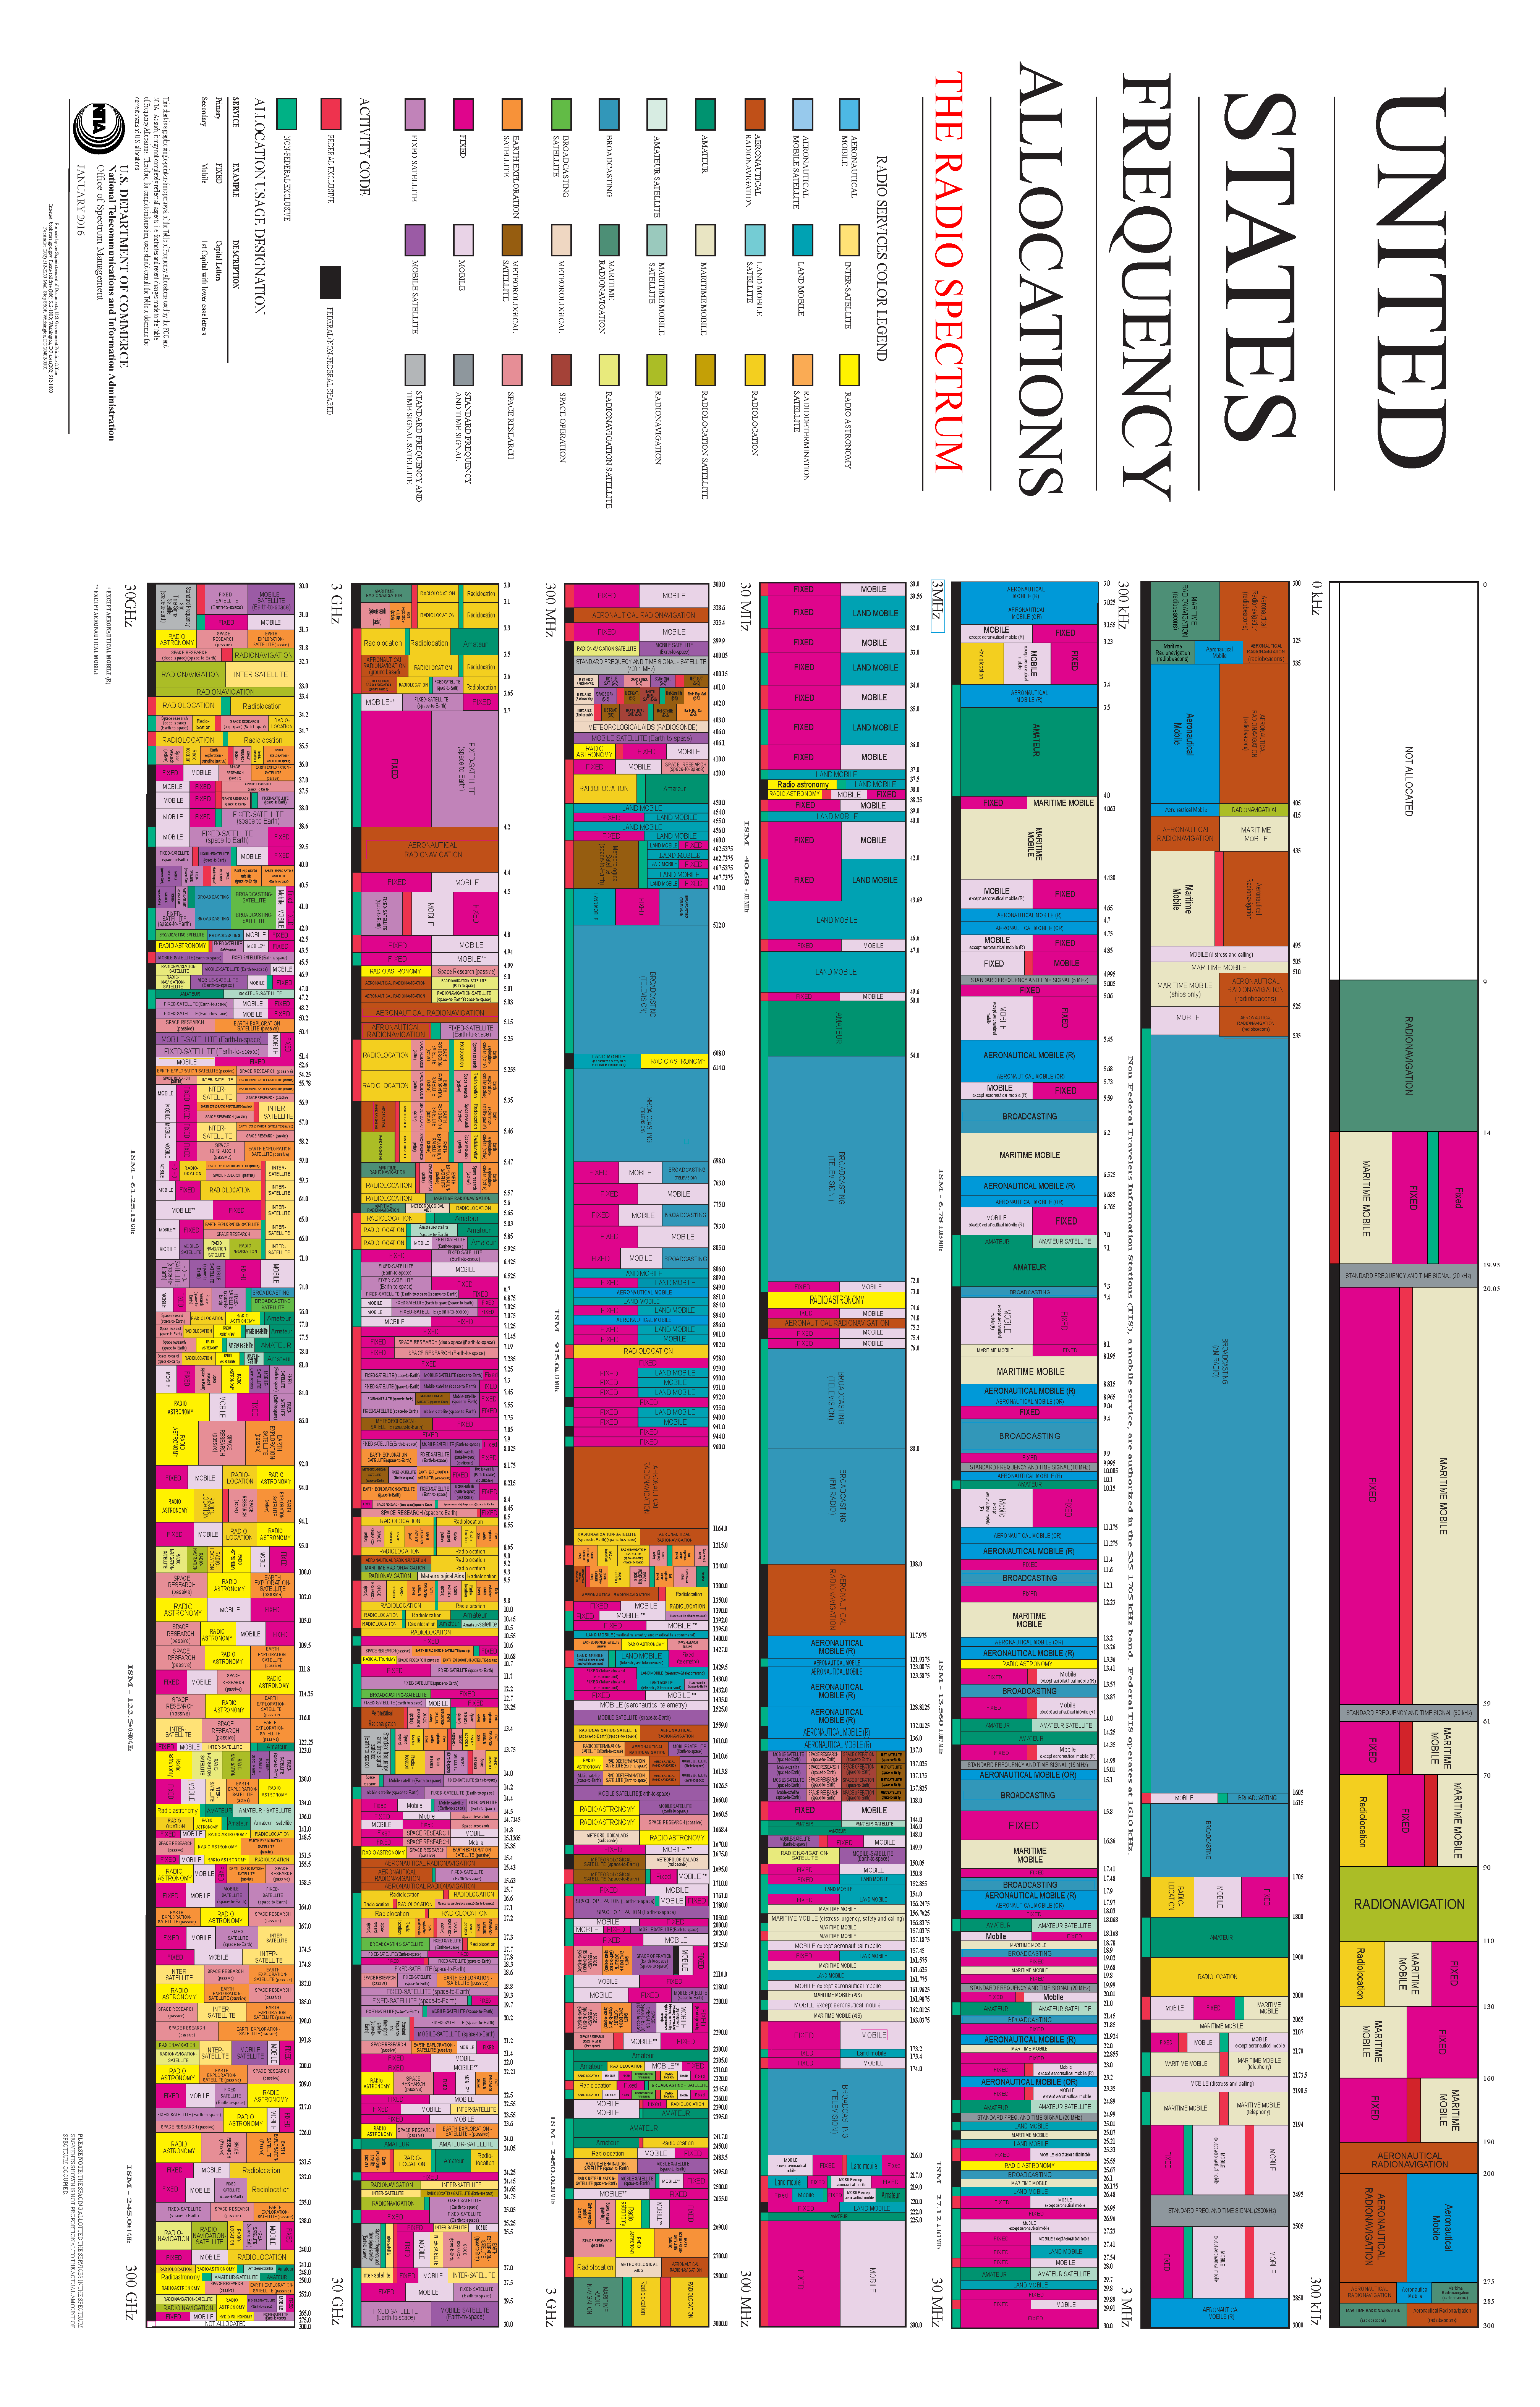
\includegraphics[width=0.65\textwidth,angle=90]{United_States_Frequency_Allocations_Chart_2016_The_Radio_Spectrum.pdf}
    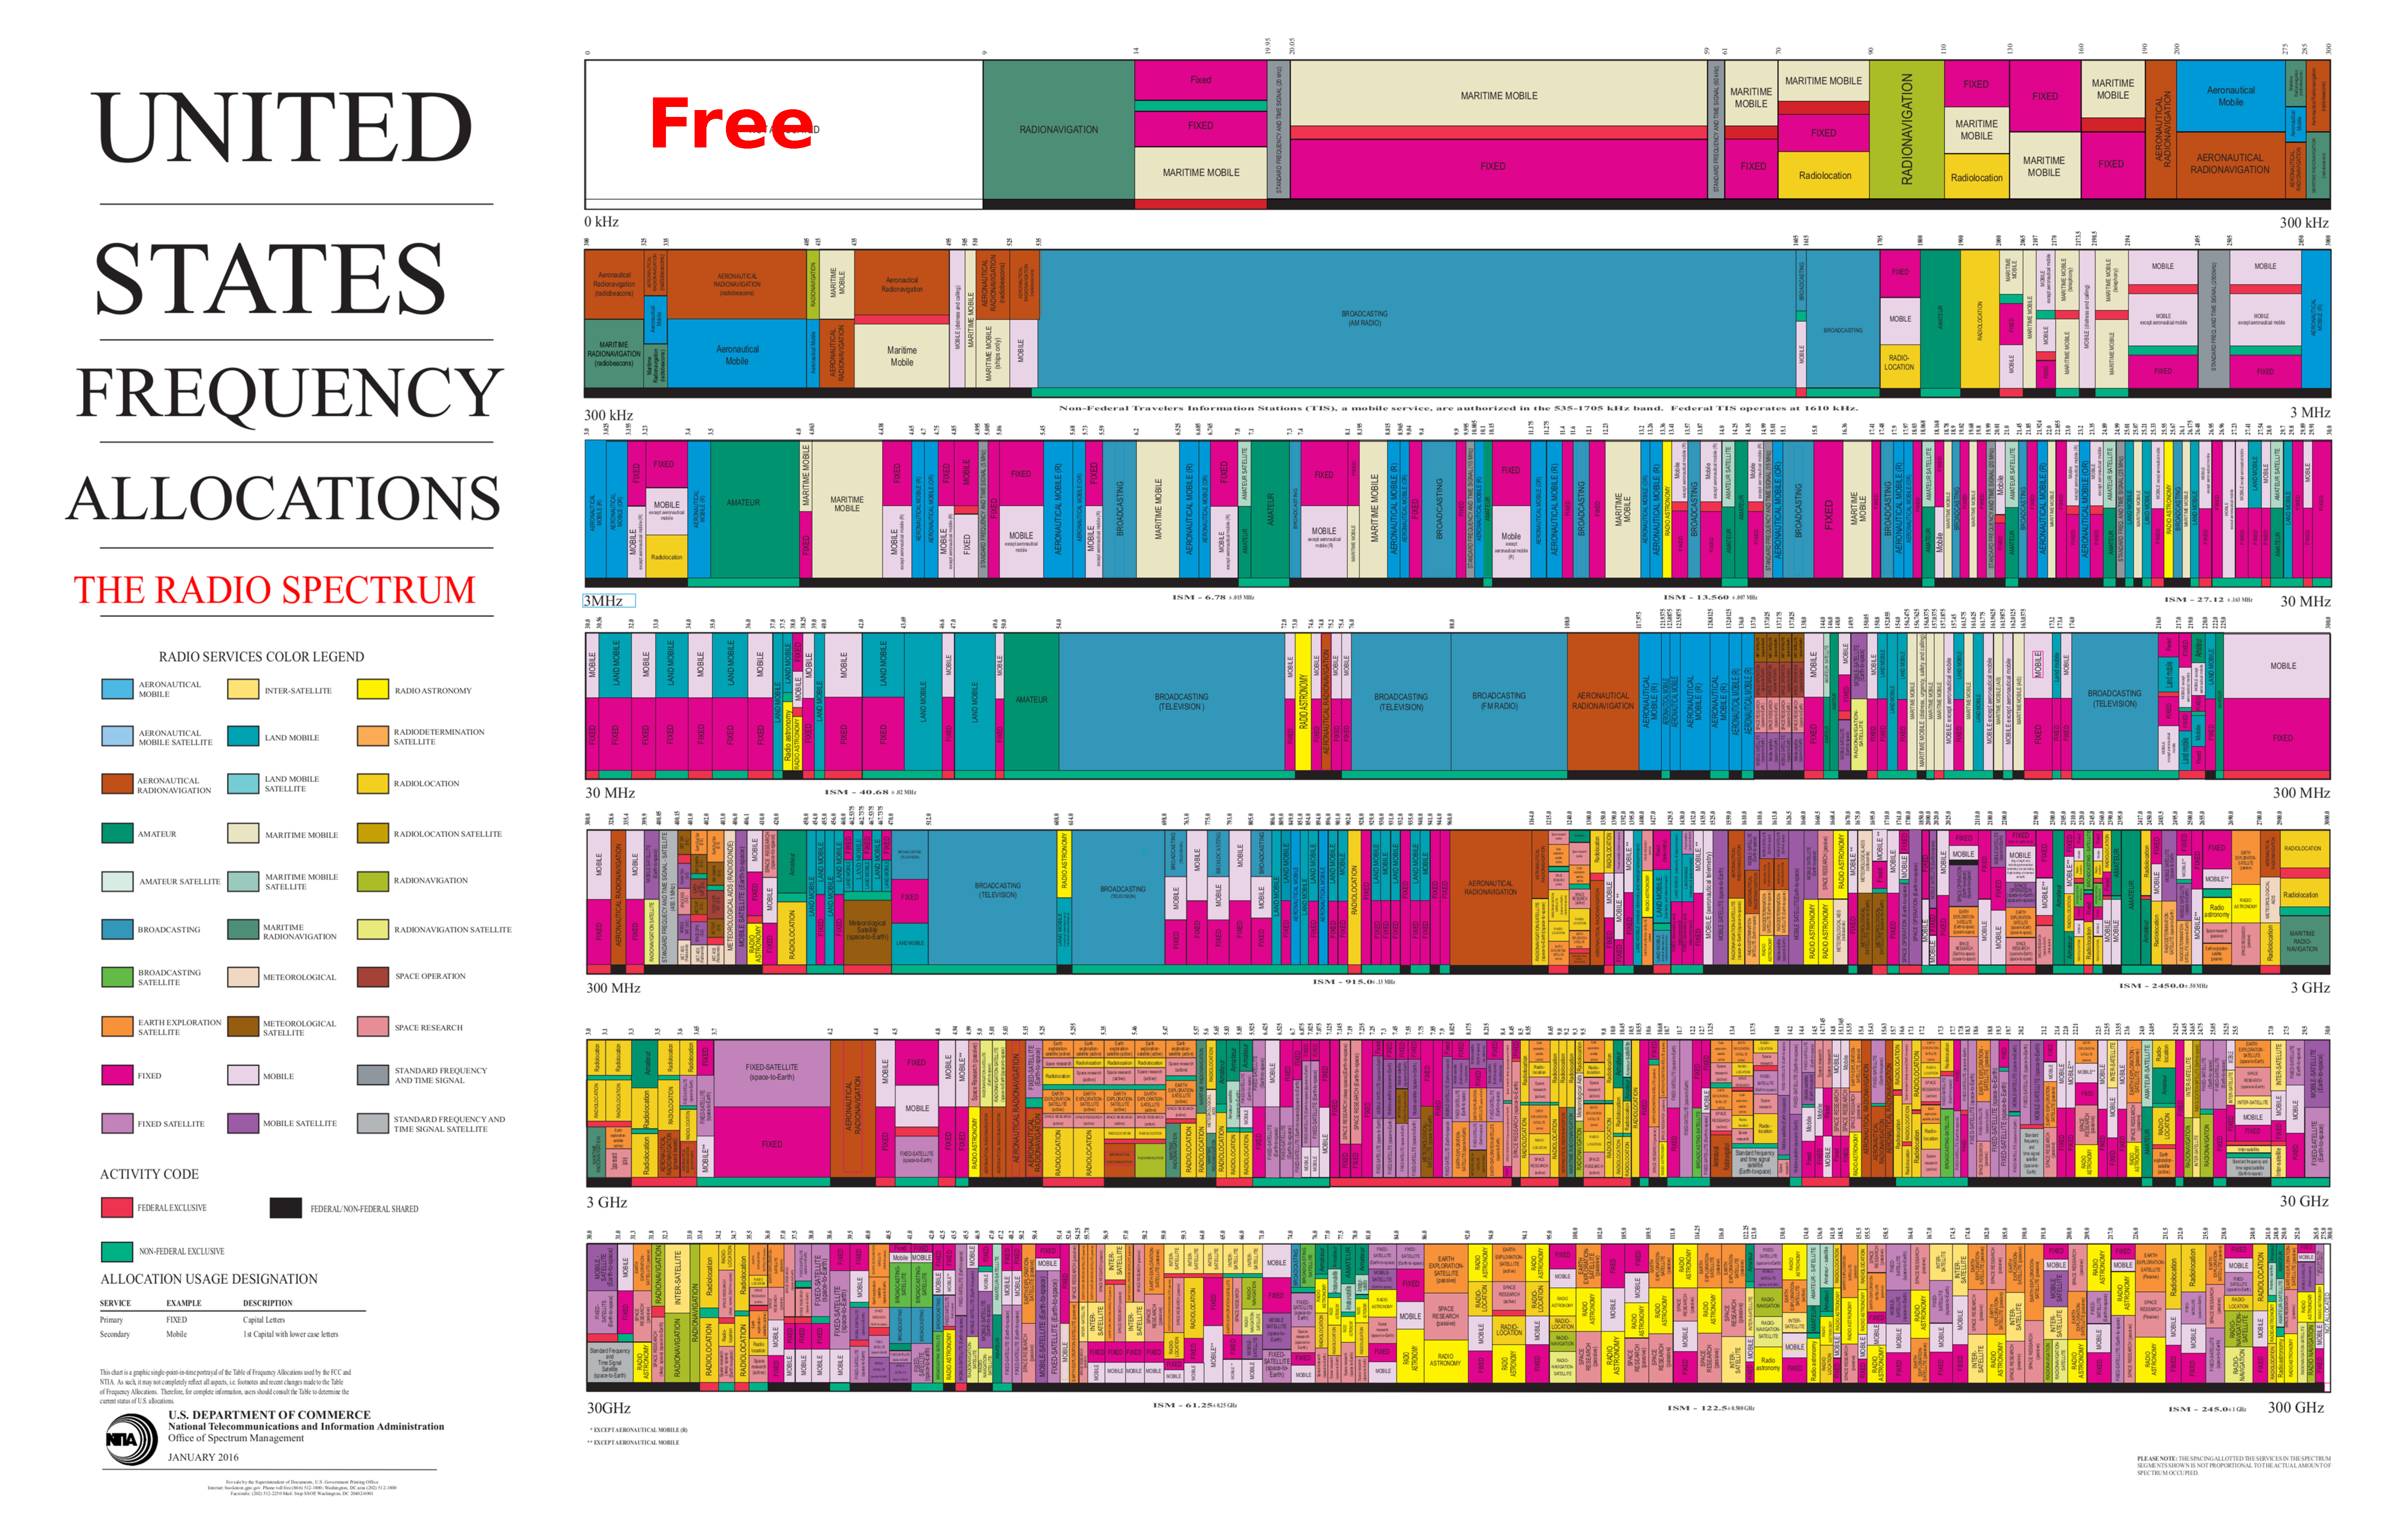
\includegraphics[width=0.99\textwidth]{United_States_Frequency_Allocations_Chart_2016_The_Radio_Spectrum_3.pdf}
    \caption[A chart representing the allocation of radio spectrum in the United States of North America in $2016$]{A chart representing the allocation of radio spectrum in the United States of North America in $2016$. \copyright{} United States of North America, Department of Commerce, published online at \href{https://www.ntia.doc.gov/files/ntia/publications/january_2016_spectrum_wall_chart.pdf}{\texttt{www.ntia.doc.gov/files/ntia/publications/january\_2016\_spectrum\_wall\_chart.pdf}}.}
    % Only a small share of the spectrum is not yet allocated, the top-left corner in white and indicated by \textcolor{red}{\textbf{Free} in red} (it is in logarithmic scale from \SI{0}{\kilo\hertz} to \SI{300}{\giga\hertz})
    % https://commons.wikimedia.org/wiki/File:United_States_Frequency_Allocations_Chart_2016_-_The_Radio_Spectrum.pdf
    % https://upload.wikimedia.org/wikipedia/commons/c/c7/United_States_Frequency_Allocations_Chart_2016_-_The_Radio_Spectrum.pdf?uselang=fr
    \label{fig:1:United_States_Frequency_Allocations_Chart_2016_The_Radio_Spectrum}
\end{figure}

Cellular network bands are overloaded in most parts of the world (2G/3G/4G/5G), but other frequency bands (such as military, amateur radio and paging frequencies) are less utilized.
Independent studies performed in some countries confirmed that observation, and concluded that spectrum usage highly depends on both time and place, as shown by \cite{Lopez2009spectral} for instance.
Moreover, the fixed spectrum allocation prevents
the introduction of new services, especially for low-cost or small markets equipment.
% rarely used frequencies, like those assigned to specific services, from being used, even when any unlicensed users would not cause noticeable interference to the assigned service.
Therefore, in the last $15$ years, thanks to an active lobbying by the cognitive radio community,
regulatory bodies all over the world have been considering whether to allow
a new wireless communication paradigm:
enable unlicensed users in licensed bands, if they would not cause any interference to the (paying) licensed users.
These initiatives are considered by the \textbf{Cognitive Radio} field that we detail below, and especially for \textbf{Dynamic Spectrum Access (DSA)},
for which we refer to the surveys \cite{akyildiz2006next,garhwal2012survey} for more details.


% \TODOL{Je peux améliorer (ou enlever) ce passage qui site J.Toledano, ou alors le commenter en plus de détails ? J'aime bien son rapport en fait (j'aurai du le lire au début de ma thèse !)}
% % https://www.economie.gouv.fr/files/files/PDF/french-spectrum-mission-executive-summary-2014-06-25.pdf
% % https://www.economie.gouv.fr/files/files/PDF/rapport-gestion-dynamique-spectre-2014-06-30.pdf
% To highlight that the spectrum scarcity is not only an issue in the USA,
% we quote the abstract of the ``Dynamic Spectrum Management For Innovation and Growth'' report by J. Toledano \cite{Toledano2014EnglishSummary,Toledano2014FrenchFull}, who was commissioned by the French government in $2014$.
% Different important problems are mentioned:
% %
% \begin{itemize}%\tightlist
%     \item
%     \emph{``In France, digital economy represents $5\%$ of GDP and affects $80\%$ of the French economy.''}
%     And the usage of wireless communications is nowadays worldwide and omnipresent:
%     \emph{``Radio frequencies are essential to many sectors: communications, broadcasting, transportation, satellite networks, energy networks and smart grids, public or private security, defense, etc.''}
%     Thus it is of highest interest to set up efficient, green, low-cost and durable new technologies for the future wireless standards, networks and devices.
%     %
%     \item
%     The radio spectrum is not only widely used for all kinds of applications, it is nowadays intensely used for some of them.
%     \emph{``Everyone agrees on the growing need for spectrum.
%     This growing need results from two phenomena.
%     On the one hand, mobile traffic should be multiplied by $13$ to $25$ fold between $2011$ and $2017$.
%     On the other hand, the development of new innovative services such as the Internet of Things and its multiple applications (smart cities, e-health...), could lead to a growing number of connected devices, up to $50$ billion in $2020$, according to estimations.''}
%     The first estimation was correct, and the mobile traffic is again \href{https://www.ericsson.com/en/mobility-report/future-mobile-data-usage-and-traffic-growth}{estimated} to be increased by $10$ times between $2019$ and $2025$.
%     % https://www.ericsson.com/en/mobility-report/future-mobile-data-usage-and-traffic-growth
%     % https://www.cisco.com/c/en/us/solutions/collateral/service-provider/visual-networking-index-vni/white-paper-c11-738429.html
%     If the second estimation was overestimating the growth of the IoT market, forecasts predict  more than 64 billion IoT devices by 2025.
%     % https://www.businessinsider.com/internet-of-things-report?IR=T
%     \item
%     \emph{``Today, there are no more available frequencies in the easily exploitable frequency bands.
%     Moreover, it is getting more and more difficult to resort to classical methods of frequency bands liberation.''}
%     As illustrated above in Figure~\ref{fig:1:United_States_Frequency_Allocations_Chart_2016_The_Radio_Spectrum}, and discussed in \cite{patil2011survey,valenta2010survey}.
%     \item
%     \emph{``Growing recourse to spectrum sharing, and in particular dynamic spectrum sharing, constitutes an important spectrum reserve.
%     A particular sharing form, the use of unlicensed bands, open to all and free, has been intensely developed with the growth of Wi-Fi use.''}
%     This thesis focusses on spectrum sharing in unlicensed bands, for IoT networks that lie at the opposite direction as the one underlying Wi-Fi networks: the spectrum sharing will be learned automatically by the end-devices, and not centrally decided by the base station.
% \end{itemize}


\section{Cognitive Radio and Multi-Armed Bandits}

In this thesis, we study Internet of Things networks characterized by mainly three essential constraints:
low power consumption (or long battery life),
long-range communications,
and low duty cycle.
%
More precisely, we study the possible interconnections between \textbf{Cognitive Radio} and \textbf{Machine Learning} applied for IoT networks.
Let us define and detail both concepts.

% This thesis studies the possible applications of a certain kind of Machine Learning algorithms, Multi-Armed Bandits, to a certain kind of Telecommunications, Cognitive Radio and Internet of Things of Networks.


% \TODOL{Émilie pense que je devrais faire ça mieux :
%     Quant au survey du machine learning (Figure 1.1), je ne pense pas que
%     cela soit nécessaire. Je trouve ça plus pertinent d'introduire le
%     problème de décision séquentielle qui nous intéresse (qui n'est pas
%     juste un sub-field du machine learning d'ailleurs, la communauté
%     statistique s'y intéresse depuis bien plus longtemps !), sur l'exemple
%     de l'OSA.
% }


\paragraph{From IT to Cognitive Radio.}
%
We can narrow down the first field of study of this thesis, steps by steps:
from Information Technologies (IT), to Telecommunications, to Wireless Communications, then to Cognitive Radio (CR),
and finally to Software Defined Radio (SDR).
%
The transition from the historical approach of hardware-based radio to SDR architectures is a gradual process, that started in the early $1990$s and has accelerated in the $2000$s.
% https://en.wikipedia.org/wiki/Software-defined_radio
A SDR is a radio communication system where components that have been traditionally implemented in hardware (\eg, mixers, filters, modulators/demodulators, detectors, etc) are more and more implemented by means of software on a processor.
%  with the exception of a unique pair of receiver/transmitter antennas.
Even though the SDR paradigm was initiated by the United States of North America defense research in the $1980$s, over the past $20$ years the civil industry has started to be interested by SDR, and CR has got significant attention from the academia as well.
% CR has been the first answer to solve spectrum scarcity issue which collected a huge attention in early 21st century.
%
As CR is not a standard technology, it does not have a single definition, so let us start by quoting the definition of two researchers whose works constitutes the roots of the development of CR, the first one having appeared just $20$ years ago.
% - technologies de l'information > télécommunications > communications sans fil > radio intelligente > DSA > OSA
%
% je peux faire comme Navik, donner des définitions de la CR, citant d'autres travaux
\begin{itemize}\tightlist
    \item
    J. Mittola in $1999$ proposed that
    \emph{``a really smart radio that would be self-, RF- and user-aware, and that would include software technology and machine learning capabilities along with a lot of high-fidelity knowledge of the radio environment''} \cite{Mitola99}.

    \item
    Then S. Haykin in $2005$ also said that
    \emph{``a CR is an intelligent wireless communication system that is capable of being aware of its surroundings, learning, and adapting its operating parameters (\eg, transmit power and carrier frequency) on the fly with an objective of providing reliable anytime, anywhere, and spectrally efficient communication''} \cite{Haykin05}.
    % He was the first to propose to use CR for Dynamic Spectrum Access.

    \item
    The \href{https://en.wikipedia.org/wiki/Cognitive_radio}{Wikipedia encyclopedia} states
    \emph{``a CR is a radio that can be programmed and configured dynamically to use the best wireless channels in its vicinity to avoid user interference and congestion. Such a radio automatically detects available channels in wireless spectrum, then accordingly changes its transmission or reception parameters to allow more concurrent wireless communications in a given spectrum band at one location''}.
    (\href{https://en.wikipedia.org/wiki/Cognitive_radio}{\texttt{en.Wikipedia.org/wiki/Cognitive\_radio}})
\end{itemize}


% explain PU and SU in a few sentences
One possible way of considering spectrum flexibility is the following.
%
In licensed bands, there are Primary Users (PU) paying to access the network, for instance anybody has to pay to have a mobile phone number and use cellular networks.
As exposed in the definition above of the CR philosophy, we could imagine that if the network is unused by any PU in a certain location and time, then non licensed users, referred to as Secondary User (SU), could use it, possibly by also paying some rent to the network operator.
%
Regulation states that PU have a strict priority,
but even though the RF bands are allocated, real world measurements often show that some bands are not densely used, and thus if a SU was equipped with an efficient \emph{spectrum sensing} capacity, it could analyze its environment, and use a licensed band if and only if it is free of any PU.
% explain DSA
This defines the concept of \textbf{Opportunistic Spectrum Access} (OSA), for which we refer to the survey \cite{Zhao07} for more details.
% After a short paragraph on Reinforcement Learning, we then focus on the OSA problem.



\paragraph{From Statistics or Machine Learning to Multi-Armed Bandits.}
%
% Similarly, we can narrow down the second field of study of this thesis, steps by steps.
% Stats > sequential learning > bandits
% A first point-of-view is the historical one, as
We are interested by Multi-Armed Bandits (MAB) learning,
which emerged as an interesting problem in the statistics community and among researchers interested by sequential learning, as shown by the pioneer works of \cite{Thompson33,Robbins52,LaiRobbins85}.
It is also included in the more general concept of Reinforcement Learning (RL), itself one of the field of Machine Learning (ML).
% ML > RL > MAB
% We can also expose another point-of-view, which starts from the general concept of Machine Learning (ML), and focus on , then on MAB learning.
% As illustrated in Figure~\ref{fig:1:MainTypesOfMachineLearning}, there are other types of ML, that we do not focus on in this thesis.
%
The reference book on RL is \cite{SuttonBarto2018}, so let us quote the definition of RL given by R. Sutton and A. Barto:
\emph{``Reinforcement learning is learning what to do - how to map situations to actions - so
as to maximize a numerical reward signal. The learner is not told which actions to
take, but instead must discover which actions yield the most reward by trying them''}.
% - apprentissage statistique (machine learning) > séquentiel > par renforcement > information partielle (bandits)



% \begin{figure}[h!]
%     \centering
%     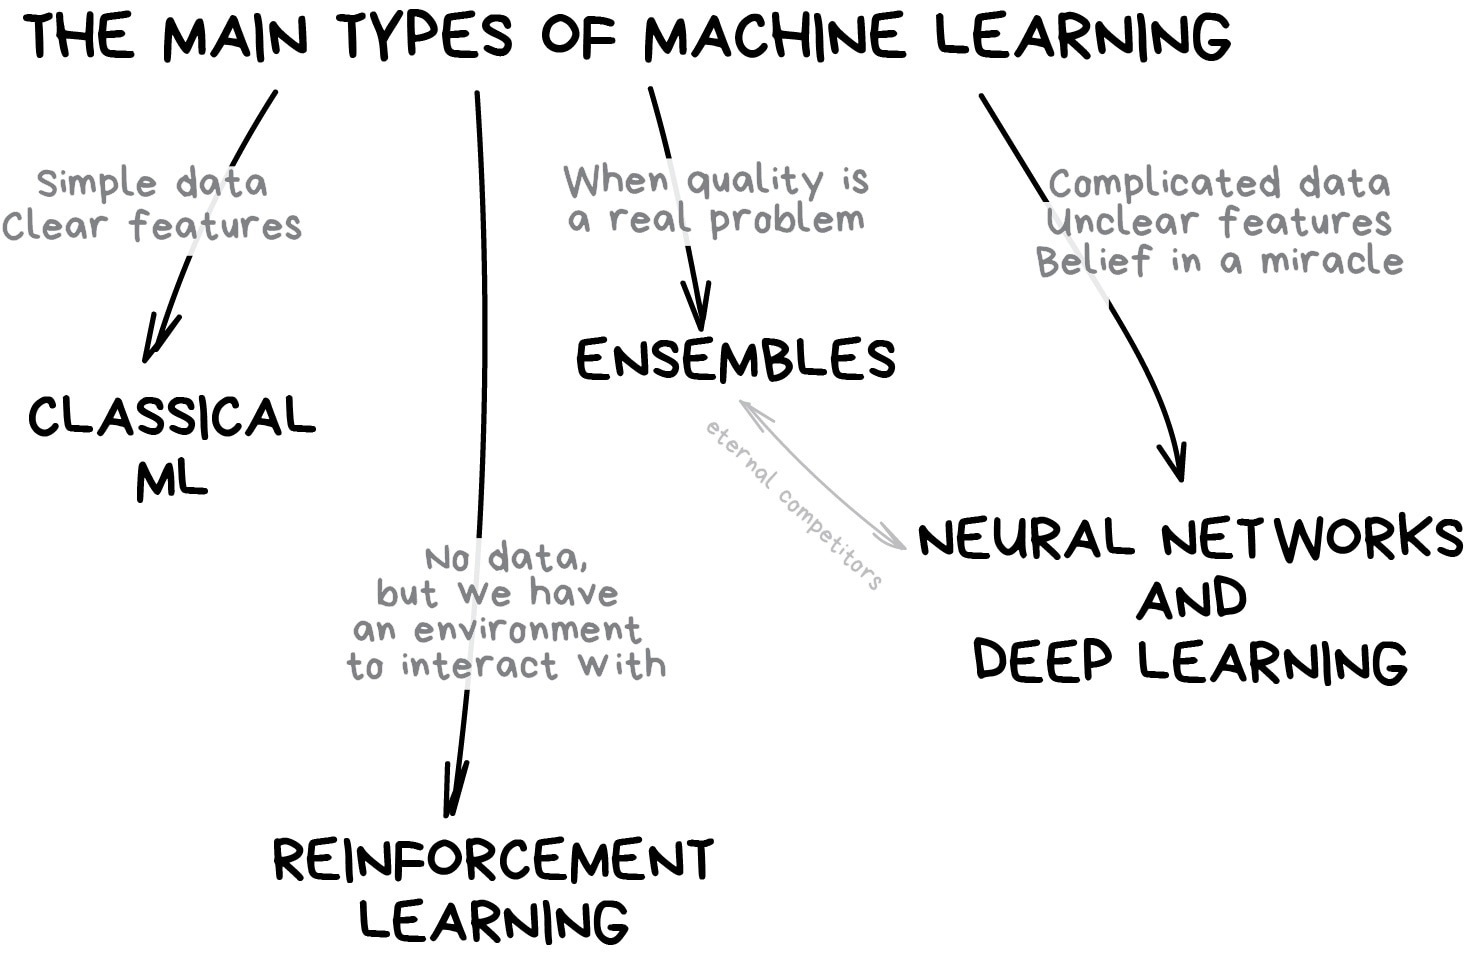
\includegraphics[width=0.45\textwidth]{Illustration_of_Machine_Learning_and_Reinforcement_Learning.jpg}
% \caption{Main types of Machine Learning, \copyright{} from \href{https://vas3k.com/blog/machine_learning/}{\texttt{VAS3k.com/blog/machine\_learning}}.}
% \label{fig:1:MainTypesOfMachineLearning2}
% \end{figure}

% % Modified from the https://draw.io/ map from
% % https://github.com/trekhleb/homemade-machine-learning/blob/master/images/machine-learning-map.xml
% \begin{figure}[h!]
%     \centering
%     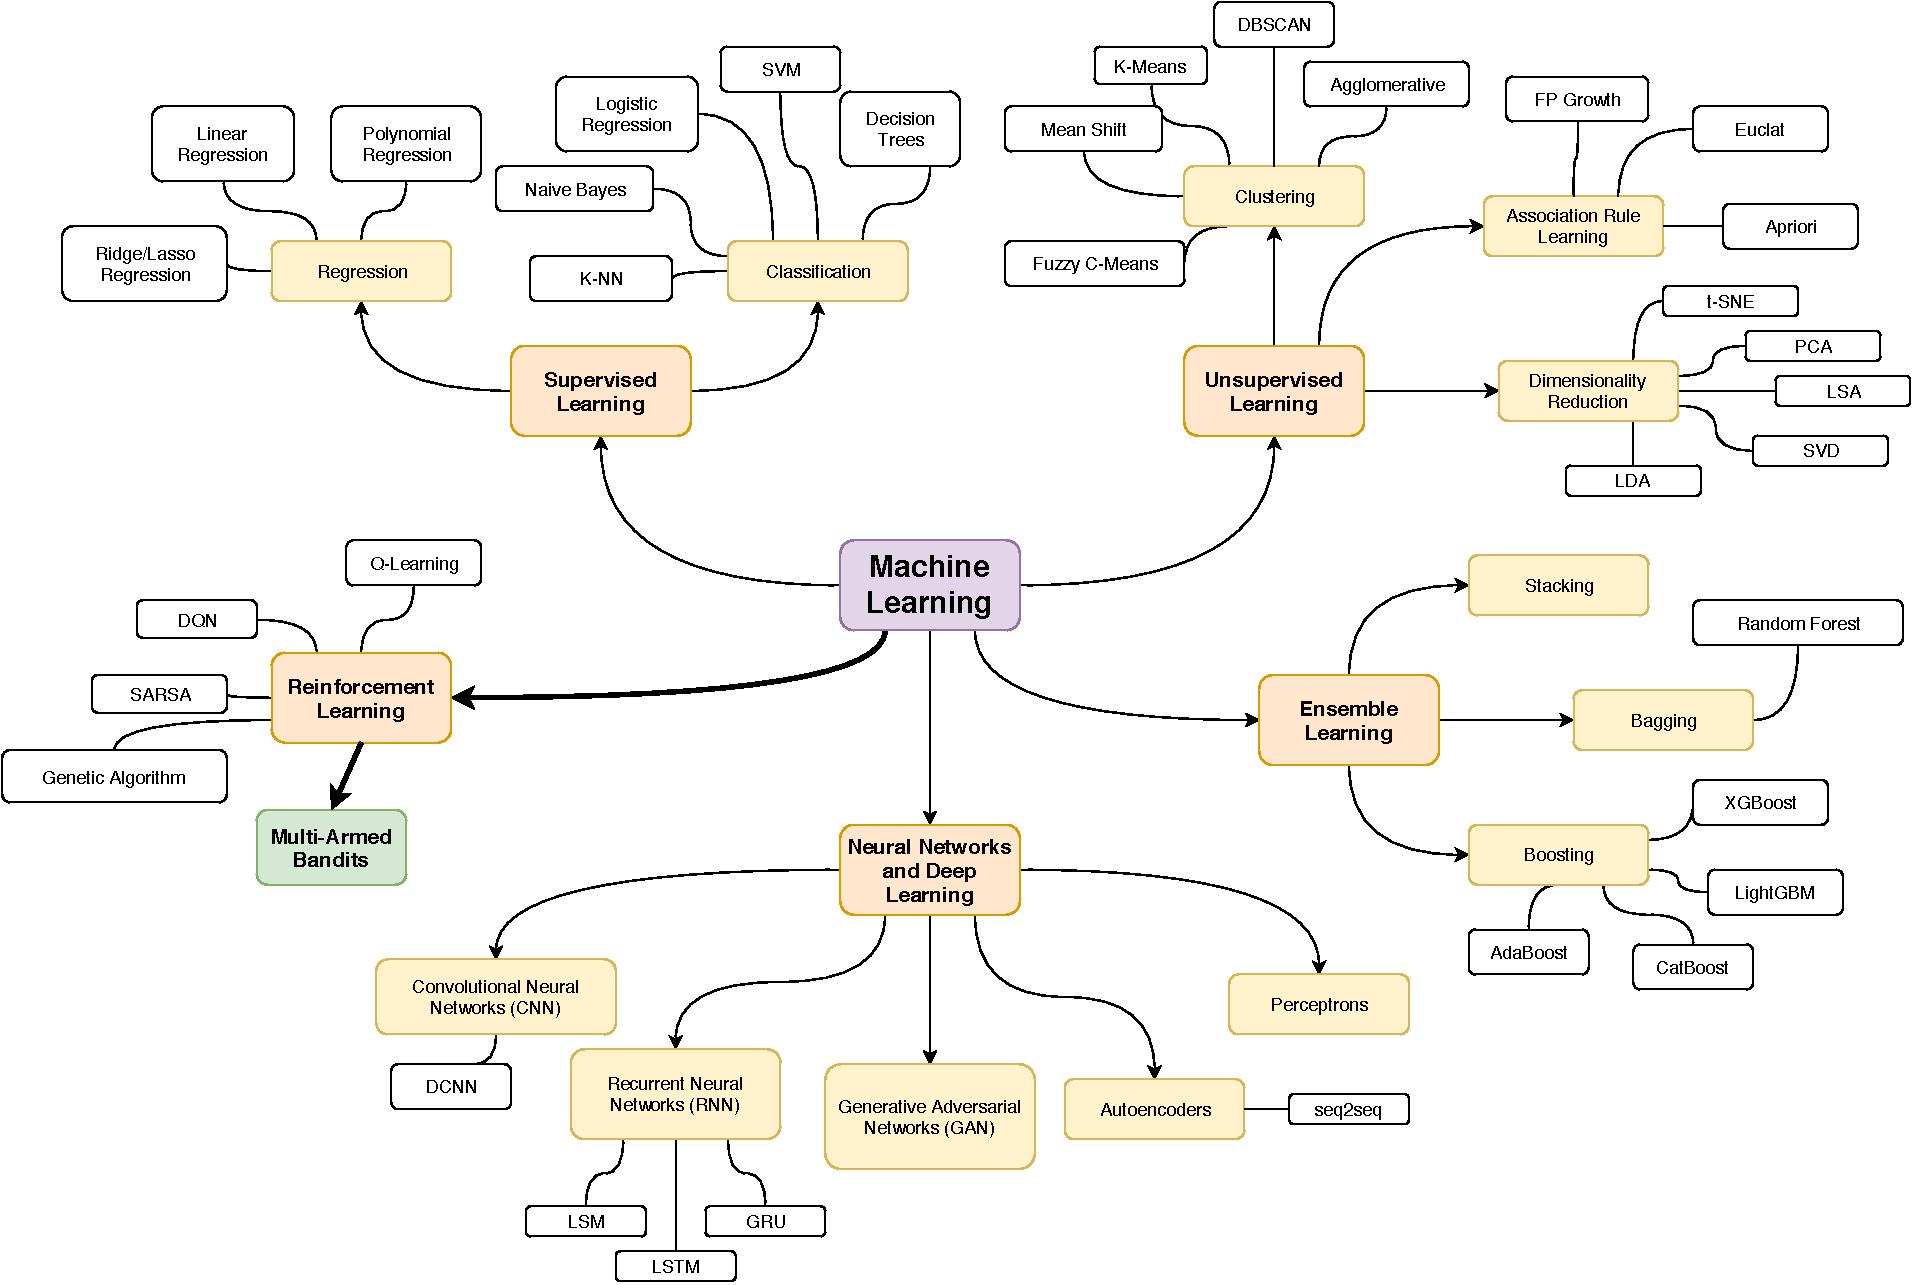
\includegraphics[width=0.95\textwidth]{machine-learning-map.pdf}
%     \caption[Classification of the main types of Machine Learning.]{Classification of the main types of Machine Learning: MAB is a subset of Reinforcement Learning and RL is a subset of ML. MAB is RL with partial information, and RL is ML with no supervision or data, just an environment to interact with.}
%     \label{fig:1:MainTypesOfMachineLearning}
% \end{figure}

We illustrate below the idea of a \emph{learning cycle}, alternating between action and feedback,
in Figure~\ref{fig:1:ReinforcementLearningCycle}.
A player (or learner) interacts with its environment by taking an action $A(t)$ (\eg, a choice in a finite set, $A(t)\in\{1,\dots,K\}$, or a vector $A(t)\in\R^d$), and then by observing a reward $r(t)$, which is a certain measure of success of this action, produced by the environment (\eg, $r(t)\in\{0,1\}$ for binary failure/success, or $r(t)\in\R$).
The goal of the player is to maximize its rewards, by trials and errors (\ie, actions and rewards).
Many real-world problems can be framed as Reinforcement Learning problems, as illustrated by the survey \cite{bouneffouf2019survey} and Section~\ref{sec:2:applicationsofStochasticMAB}, for instance learning to walk, to drive, to play a board or computer game, discovering which treatment is efficient in healing a certain disease (clinical trial), etc.

% \begin{figure}[h!]
%     \centering
%     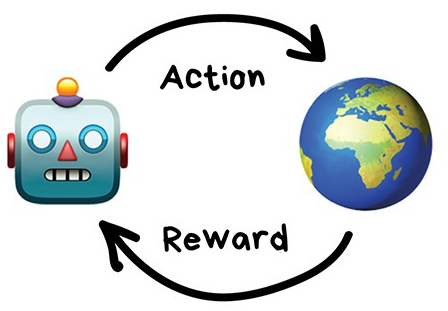
\includegraphics[width=0.25\textwidth]{Illustration_of_Reinforcement_Learning_action-reward_loop.png}
%     \caption{Reinforcement learning cycle, a learner interacts with its environment through actions, and observes a reward, iteratively. \copyright{} from \href{https://vas3k.com/blog/machine_learning/}{\texttt{VAS3k.com/blog/machine\_learning}}.}
%     \label{fig:1:ReinforcementLearningCycle}
% \end{figure}

\tikzstyle{block} = [align=center, draw, fill=gray!25, rectangle, minimum height=3em, minimum width=6em]
\begin{figure}[h!]
    \centering
    \resizebox{0.30\textwidth}{!}{
        \begin{tikzpicture}[auto,node distance=5cm,>=latex,scale=1.5]
            %
            % We start by placing the blocks
            \node [block] (player) at (0,0) {Player};
            % We draw an edge between the player and system block to
            \node [block] (environment) at (2,0) {Environment};
            % Once the nodes are placed, connecting them is easy.
            \draw [->] (player) to[bend left=90] node[pos=0.5] {Action} (environment);
            \draw [->] (environment) to[bend left=90] node[pos=0.5] {Reward} (player);
            %
        \end{tikzpicture}
    }
\caption{Reinforcement learning cycle: a learner interacts with its environment through actions, and observes a reward, iteratively.}
\label{fig:1:ReinforcementLearningCycle}
\end{figure}


% Il faut expliquer ce que c'est que les bandits, rapidement, et leur application à l'OSA
As this thesis focuses on Reinforcement Learning models,
it is important to highlight that in such decision making models, the learner does not have access to the entire reaction of the environment after taking its action.
%
In other words, the player only sees the reward generated by playing its action at every round, and not the reward that would have been given if she chose any other action.
This kind of limited feedback is called \emph{bandit information}, and we discuss the history and the concept of MAB in details in the next Chapter~\ref{chapter:2}.
Clinical trials and treatment discovery were historically the first application of MAB since the $1930$s, with the early work of W. Thompson \cite{Thompson33},
%
as MAB are indeed a simple yet powerful example of the well-known \emph{exploration vs exploitation dilemma}.
When facing a set of $K$ actions whose effects on the environment are unknown, a learner must balance between
exploring the unknown actions, in order to collect more information about them,
and exploiting the best action, according to its current knowledge.
%
The MAB problem has been studied in both the machine learning and the statistics communities, since the $1950$s with pioneers like H. Robbins \cite{Robbins52}, and more recently it is an active field of research, since the late $1990$s \cite{Anantharam87a,Anantharam87b,auer1995gambling,Agrawal95}.
The research on MAB has produced a vast literature in the $2000$s \cite{Auer02,Auer02NonStochastic,Audibert2009minimax} and continues to be a topic of high interest, as illustrated by the surveys and books \cite{Bubeck12,LattimoreBanditAlgorithmsBook,Slivkins2019}, and the wide range of applications of MAB in the recent years \cite{bouneffouf2019survey}.


\paragraph{Opportunistic Spectrum Access.}
%
The two communities of OSA and MAB have started to interact, and the resulting works have received a great interest from both communities, since the late $2000$s and early $2010$s, with pioneers works like \cite{Liu08,Zhao10,Jouini09,Jouini10}.
The focus is on one SU accessing a licensed spectrum, occupied by PU that have a strict priority over the SU, which has to follow a ``listen-before-talk'' access scheme.
%
The following hypotheses are made:
the SU is equipped with a spectrum sensing capability,
and considers a fixed and finite set of $K$ orthogonal channels, \ie, different frequency bands in a licensed spectrum.
For instance, it can be a set of $K=3$ Wi-Fi channels at different frequencies, emitted by the same Wi-Fi station.
Another hypothesis is that both PU and SU are synchronized in time, by sub-dividing the time in discrete time steps (or rounds).
%
Thus if the SU spends a short time in the beginning of each time slot to perform sensing, it can scan for the presence or absence of any PU before transmitting, without colliding with the PU during the rest of the time slot.
If the SU was able to sense for all the $K$ frequency bands, it could simply transmit in one of the free channels if any, or not transmit if all channels are used at a given time step.
However, sensing is known to be costly, in terms of energy consumption, especially for wide-band sensing, as detailed in the surveys \cite{yucek2009survey,subhedar2011spectrum}, thus most works on OSA limit the sensing capacity of SU to sensing only one channel at a time.
This assumption, along with the hypothesis that PU cannot be disturbed (without which no regulation will ever be accepted for OSA), enforces the SU to transmit in the channel that it sensed, if and only if it was sensed free from any PU.
% non negligible cost of radio reconfiguration

Focusing on one SU in an OSA network, it has to sequentially decide a channel to sense (in the set of channels, $[K]=\{1,\dots,K\}$), then it performs spectrum sensing, and finally it transmits in this channel if it was sensed free.
The goal of the SU is to minimize its energy consumption (we remind that we focus on ``green'' cognitive radio) and to maximize its up-link data rate, or equivalently, to maximize its number of successful transmission.
%
If the different channels are not uniformly used by the PU, and if we assume a stationary hypothesis on the PU traffic, then the goal of the SU boils down to exploring the different channels and exploiting the best ones.
This frames the Opportunistic Spectrum Access problem as an exploration/exploitation problem,
with a finite set of actions (the channels, also called \emph{arms}),
in a sequential action-then-feedback cycle (time steps are $t\in\N^*$),
under partial information feedback (\ie, the player receives sensing feedback about only one channel over $K$).
These three hypotheses are the ones that restrict from the general sequential learning framework to the specific MAB case (see Figure~\ref{fig:1:ReinforcementLearningCycle}).


\paragraph{MAB for OSA, and a short history of these researches at the SCEE team.}
%
Previous works of our SCEE team showed that MAB can be used to model the OSA problem:
orthogonal frequency bands (or channels) are modeled by arms $k\in\{1,\dots,K\}$,
and the feedback obtained by the CR-equipped device after sensing the channel $k$ at time $t$ is modeled by a reward of $r(t) \in \{0,1\}$.
Indeed, $r(t) = 1$ indicates that no Primary User was sensed (and thus the SU can send a message), while a reward of $r(t)=0$ indicates that the channel $k$ is busy during the time slot $t$, and no message should be sent, until the end of that slot.
%
This model was first studied by W. Jouini during his PhD thesis with C. Moy \cite{Jouini12PhD}, about ten years ago, first in the article \cite{Jouini09} and later in \cite{Jouini10,Jouini12}.

Their works were among the first ones to propose to use Reinforcement Learning for Cognitive Radio and the OSA problem, especially the MAB model and the $\UCB_1$ algorithm,
along with the early works of Q. Zhao and her team, for instance with \cite{Liu08,Zhao10}.
%
Shortly after in $2014$, proof-of-concepts using real-world radio hardware and Software Defined Radio were developed by C. Moy and his student C. Robert, using USRP boards and the MATLAB/Simulink software \cite{RobertSDR2014,MoyWSR2014}.
In a second PhD thesis, N. Modi studied from $2014$ to $2017$ the impact on the battery life of a wireless device of using MAB algorithms to optimize channel selections \cite{Modi17PhD}.
% On the one hand, running a MAB algorithm such as UCB-like algorithms was proven to be useful and could bring significant improvement in terms of successful transmission rates, directly increasing the battery life of the device.
% On the other hand, classical MAB algorithms tend to switch arms a lot of times, especially in the beginning of their learning process, and this induces a lot of dynamical hardware reconfigurations for the wireless device, as selecting a different channel requires a change in the radio hardware used by the device.
% Each hardware reconfiguration costs energy for the device, and so quickly-switching algorithms lead to a reduction of the battery life.
The trade-off between rapid software reconfigurations that cost energy but allow to learn quickly is studied empirically in \cite{modiDemo2016}.

In $2017$, C. Moy continued to work on this direction, with a post-doctoral student, S. Darak, leading to publications such as
\cite{darak2016bayesian,Darak16}.
%
For example, proof-of-concepts like \cite{kumar2016two} have proven the capability of such approaches on real radio signals for OSA.
%
Some analysis on real radio measurements made for HF ionospheric channels have also proven that solutions based on MAB learning are appropriate, and solve efficiently this kind of decision-making problems on real-world wireless signals \cite{Melian15}.
%
Since $2017$, S. Darak, and his team at IIIT Delhi in India, have actively worked in the research on cognitive radio using multi-armed bandits.
Inheriting from his work with the SCEE team,
some of their recent works are also illustrated with realistic demos using USRP and the MATLAB/Simulink system
\cite{KumarYadav2018,SawantKumar2018,JoshiKumar2018}.
%
For more details on the state of research on Cognitive Radio, we refer to the surveys \cite{garhwal2012survey,marinho2012cognitive}.

% \TODOL{Raccourcir toutes les fois où je parle des travaux sur l'OSA après dans la suite de la thèse !}


\paragraph{Limitations and specifities of IoT networks.}
%
The aforementioned literature has essentially shown that MAB algorithms can be applied successfully on the SU side for the OSA problem.
However, if we consider CR-ready devices that cannot perform spectrum sensing, such as low-cost and low energy-consumption end-devices designed for the future Internet of Things networks, the MAB model that uses sensing to detect PU in the OSA case can no longer be applied.
Moreover, in most cases, the IoT networks use unlicensed bands, and as such there is no longer a distinction between PU and SU.
In other words, there is no longer any priority between users in IoT networks.
%  (no more PU, all are SU).
%
The other specificities of IoT networks can be listed as follows,
and we refer to the survey \cite{Centenaro16} for more details.
\begin{itemize}\tightlist
    % \item
    % we consider here IoT networks that run in unlicensed bands (no more distinction between PU and SU),
    \item
    most IoT devices are very low-cost devices, run on low-quality hardware, and have limited software and power capabilities (\ie, tiny batteries).
    It means that even if they are not equipped with particular spectrum sensing capabilities,
    they are equipped with a transmitter as well as with a receiver (Tx and Rx, \ie, a transceiver),
    and they have low-complexity storage and computation capabilities (\ie, small embedded processors),
    \item
    a single IoT base station will have to handle a very large number of devices,
    and cannot send coordination orders to them in order to optimize the network,
    \item
    IoT devices have low to very low duty cycles (few messages every minute to only a few every month), and are in charge of initiating their up-link communications.
\end{itemize}

A central coordination of the devices with their base station is thus impossible as it would require them to communicate continuously with the base station, which violates the two last constraints.
%
Moreover, due to both their limited hardware (Rx/Tx), limited computational power and limited battery life, the IoT devices are able to use their received antenna to sense one channel occasionally (typically, for a few time slots after every single up-link message), but they cannot perform spectrum sensing like it is considered for OSA and CR (\ie, at the beginning of a time slot, in a ``listen-before-talk'' scheme).

One could think that in the absence of sensing, Reinforcement Learning is no longer possible, but any real IoT device still receives some information about its environment after some or every of its transmissions.
In most IoT standards an up-link message sent to a base station can be followed by a down-link message sent back by the base station, to indicate if the up-link message was successfully received and understood.
%
By using this feedback, which consists in an \emph{acknowledgement} (\Ack) message received shortly after every successful transmission, or in an absence of \Ack{} after a failed transmission, it is possible that an IoT end-device can also use a well-designed RL algorithm, in order to optimize its communications.
%
% To the best of our knowledge, this direction of research has never been studied before the year $2016$ and the beginning of this PhD.

% \newpage % WARNING

% ----------------------------------------------------------------------------
\section{Our contributions}
\label{sec:1:contributions}

We start by formulating the problem studied in this thesis, and then we develop the organization of the contributions.
%
% \textbf{Problematic.}
%
If we sum-up the studied problems and summarize them in one question, it could be the following:
\emph{``Can we adapt the decision making tools, already successfully applied to Cognitive Radio for Opportunistic Spectrum Access, to the specific needs of CR for the (future) Internet of Things networks?''}
%
We answer partially to this problematic by the following steps.


% \subsection{Focusing on MAB algorithms}
% \subsection{Exploring the literature of MAB algorithms}
\subsection{Exploring the Jungle of MAB algorithms}

% \paragraph{Chapter~\ref{chapter:2}.}
%
We started by exploring the rich literature of multi-armed bandits,
as many different algorithms exist, with lots of variants on the simple problem presented above.
% (see \cite{LattimoreBanditAlgorithmsBook,Slivkins2019} for surveys).
We thus start the first part of this thesis with Chapter~\ref{chapter:2}, which presents the MAB model and reviews the most important algorithms designed to solve stochastic and stationary MAB problems.
%
In order to clearly understand which algorithms could be adapted to the aforementioned constraints of CR for IoT networks,
we were not only interested by the usual measure of performance of any MAB algorithm (its regret, see below in Section~\ref{sec:2:lowerUpperBoundsRegret}),
but also by their empirical performances in terms of computational complexity and storage requirements, from the points of view of both theoretical analyses and real-world measurements.
%  on time and memory footprints.


% \paragraph{Chapter~\ref{chapter:3}.}
%
Our exploration of the large number of MAB algorithms and models developed in the recent literature
has given us the ambition to write a single software allowing anyone to easily implement new models and algorithms, in order to compare the existing ones and empirically explore the performances of newly proposed algorithms.
To tackle this goal, we developed a library of simulation of MAB problems, in the Python language.
%
To the best of our knowledge, we wrote the most exhaustive open-source library for bandits. Our library SMPyBandits is published online, under an open-source licence \cite{SMPyBanditsJMLR,SMPyBandits}, and hosted on \href{https://GitHub.com/SMPyBandits}{\texttt{GitHub.com/SMPyBandits}}.
We present in details its architecture and its features in Chapter~\ref{chapter:3}, along with different examples of its usage.
A full documentation is available online, as well as exhaustive instructions to reproduce the simulations presented in the rest of this thesis.


% \paragraph{Chapter~\ref{chapter:25}.}
%
Because there are so many MAB algorithms available, we are also interested by the question of how an engineer can choose the algorithm to implement, in a given IoT object, in order to equip this object with the capacity to adapt robustly to any environment.
To answer this question, we present two approaches.
The first one is an empirical comparison of the most efficient and well known existing algorithms, in Sections~\ref{sec:3:reviewSPAlgorithms} and \ref{sec:3:timeAndMemoryCosts}.
We confirm that widely used and not too sophisticated algorithms, such as \UCB{} \cite{Auer02}, Thompson sampling \cite{Thompson33} and \klUCB{} \cite{KLUCBJournal}, are the most efficient in terms of regret, and offer a good balance between regret and (time and memory) complexity.
The second approach is online algorithm selection, consisting in aggregating a (finite) set of algorithms and automatically discovering which one performs the most efficiently, against a given problem, with our contribution \Aggr{} that we detail in Chapter~\ref{chapter:25}.
This work on aggregating MAB algorithms was motivated for the OSA case of CR, where many previous research works only considered the $\UCB_1$ algorithm without really justifying their choice.
This contribution was presented in the IEEE WCNC conference in Barcelona, Spain, in April $2018$.


% \subsection{Focusing on IoT networks.}
\subsection{Two models of IoT networks and decentralized MAB}

In the second part of this thesis, we start by proposing and studying different models of IoT networks, with simulations and a real-world proof-of-concept, and then we study interesting questions on two mathematical models of MAB, arising from simplification of our first model.


% \paragraph{Chapter~\ref{chapter:4}.}
%
We study two models of IoT networks in Chapter~\ref{chapter:4}.
The first model considers IoT devices that simply have data to regularly send to a base station, at unpredictable or random times.
Such devices use acknowledgements as feedback, in order to optimize their up-link communications, by accessing more the best channels, \ie, the channel less occupied by the surrounding traffic.
The goal of this first model is to increase the Quality of Service (QoS) of such IoT network, by applying decentralized RL on the device side in order to reduce the rate of failed transmissions.
The base station will thus receive more up-link packets from the devices being served, if they can successfully learn by themselves an efficient spectrum access scheme.
It implies that the network can serve more end-devices while maintaining the same QoS.
%
Our second model then considers packet retransmissions, and while the two models are similar, the application of an efficient decentralized learning algorithm now results in both an increased battery life for each of the devices, and an increased QoS for the entire network, as less retransmissions reduce the local spectrum load.

% We present in Section~\ref{sec:4:firstModel} a first model of an IoT network, that is made of thousands (or more) of end-devices and a single base station.
% We consider an ALOHA-based protocol, slotted in both time and frequency, by assuming a simple pre-agreed synchronization between all devices and the base station. This synchronization is the only aspect of the network that requires central control from the base station, and it only requires one down-link packet when a new device joins the network operated by this base station \cite{Centenaro16}.
% %
% Our IoT network model contains two types of devices: \emph{static devices} that use only one channel (fixed in time), and \emph{dynamic devices} that can choose the channel for each of their transmissions.
% Static devices form an interfering traffic, which could be generated by devices using other standards as well.
% Dynamic devices can use RL, and especially MAB algorithms, to optimize their sequential choice of channels, in order to maximize the number of successful up-link transmissions, thanks to the success/failure feedback that is the presence/absence of acknowledgement (\Ack) received from the base station.
% %
% We first detail three base-lines, a naive approach and two centralized ``oracle'' approaches,
% that are used to evaluate the performance of the considered MAB algorithms (\UCB{} and TS), in terms of the centralized system-wide successful communications rate.
% We show that our approach is interesting, as these low-cost MAB algorithms have near-optimal performance, even when the proportion of end-devices increases and the interfering traffic from the other devices becomes more and more fluctuating and unpredictable.
% %
% Even without changing anything on the level of the considered IoT standard (neither the PHY nor the MAC layers), our proposal is just an add-on capability, that can be set-up on each device, on a unit-per-unit basis.
The model without retransmission comes from the first article written during this thesis, which initiated a collaboration with R. Bonnefoi, another PhD student of our team SCEE.
We presented it at the EAI CROWNCOM conference in Lisboa, Portugal in September $2017$, where it obtained the ``best paper award'' \cite{Bonnefoi17}.
%
% Verifying the potential gain of performance brought by these MAB algorithms in numerical simulations was a first step, but it is satisfactory to also verify our results on a real-world proof-of-concept (PoC).
% In Section~\ref{sec:4:firstModel}, we detail what we believe to be the first PoC of using decentralized MAB learning in a simplified IoT-like wireless network.
% We implemented a network with a base station, which receives incoming messages from different end-devices and replies with acknowledgements.
% % , that are used as feedback by the devices and let them learn an efficient spectrum access scheme.
% % Verify this first model empirically: proof of concept
The proof-of-concept (PoC) continued the fruitful collaboration, and was demonstrated during three days at the IEEE ICT conference in Saint-Malo, France, in June $2018$ \cite{Besson2018ICT}, and later at the IEEE WCNC conference in Marrakech, Morocco, in April $2019$ \cite{Besson2019WCNC}.
%
% We then consider an extension of our first model, following the idea of packet retransmissions, that is at the root of the famous ALOHA protocol \cite{Abramson1970,Roberts75}.
% The idea is that when a device sends an up-link message but does not receive its \Ack{} (before a certain delay), instead of going back to sleep mode in order to wait for its next activation (\eg, following the Bernoulli random activation pattern, or waiting for the application to need to send some data), the device will try again to send the same packet, a few times (\eg, up-to $m \leq 10$ times), after some small random waiting times.
% %
% We propose to also use decision making, that is to also use RL and MAB algorithms, for this other model, at the second layer of the MAC protocol, in order to learn the best channels to use for retransmitting the packets that suffered from a collision at their first transmissions.
% We present the model in Section~\ref{sec:4:retransmissions}, along with mathematical justifications of the potential of using this second-stage MAB learning for retransmissions, and numerical illustrations.
% This shows that using learning in a decentralized way on the devices' side is again a powerful idea under this model with retransmissions, and we show as well that the simplest of the different heuristics we compared is efficient, and allows the devices to learn to behave almost optimally.
The second model with retransmissions concluded our collaboration with R. Bonnefoi, and resulted in a paper presented in the $1^{\text{st}}$ MoTION workshop, also during the IEEE WCNC $2019$ conference \cite{Bonnefoi2019WCNC}.


% \paragraph{Chapter~\ref{chapter:5}.}
%
In both models of IoT networks presented above, the core idea is to let every dynamic device run a learning algorithm in a fully decentralized way, in order to optimize the entire system.
We highlight that each device communicates, and thus learns, only at some rounds and not at all the time steps, by following its own random activation process (we restrict to a purely random Bernoulli activation process of probability $p$).
This means that each of them target its own local objective, which is to maximize its cumulated reward, in a selfish way and by being agnostic about the other devices following the same objective.
It is well known in game theory that playing selfishly can be disastrous for the centralized performance measure, one can think of popular ``dilemmas'', such as the \href{https://en.wikipedia.org/wiki/Prisoner%27s_dilemma}{prisoner dilemma}.
% , and for more examples we refer to the book \cite{CesaLugosi06}.
% https://www.ii.uni.wroc.pl/~lukstafi/pmwiki/uploads/AGT/Prediction_Learning_and_Games.pdf
So it was quite surprising that the numerical simulations, as well as the realistic PoC, showed that decentralized selfish MAB learning leads to efficient coordination between devices in all the considered scenarios, despite the fact that these IoT objects cannot communicate directly with each other, and receive only a collision feedback from the base station they are associated to.

That is why we first tried to analyze the performance of this decentralized algorithm, that we refer to as \Selfish, in the model of Section~\ref{sec:4:firstModel},
but due to the random number of active devices at each time step (\ie, as soon as the probability $p$ of activation is $p < 1$), we were unable to develop a clean analysis.
%
That is the reason why we relax the hypothesis of having $M \gg K$ (or even simply $M > K$) devices in a network with $K$ orthogonal wireless channel in Chapter~\ref{chapter:5}, that is equivalent to having $p < 1$, and we consider the case of IoT devices communicating at every time step (\ie, $p=1$), and so we restrict to only up-to $M \leq K$ devices.
The model we studied comes with different variants, depending on the feedback level, and covers both the OSA case (\ie, with sensing of PU) or the IoT case (\ie, without sensing).
The goal was to understand the heuristic of Chapter~\ref{chapter:4}, \Selfish, in the simpler framework of multi-player MAB, which has been studied before for the case of OSA, for instance by \cite{Zhao10,Anandkumar10,Anandkumar11}.
%
The OSA case covered by the studied model can seem to slightly differ with the one exposed above, from \cite{Jouini10} and other previous works,
as our model requires that an \Ack{} is sent back by the base station if the transmission was successful, even in the case where sensing information is available.
It is actually equivalent to the previously studied models of applying MAB for OSA, as they only considered synchronized devices, only one SU and PU, and thus if the sensing indicates that one channel is free at one time slot, the up-link message sent by the SU device is sure to be successfully received by the base station (in the ideal model), so there is no risk of collision, and thus no need for an \Ack.


On the one hand, in the OSA setting, we failed to obtain positive result for the \Selfish{} policy, as we proved that in some limited settings (\eg, $K=3$ channels and $M=2$ devices), \Selfish-\UCB{} can suffer from linear regret with a small probability, and thus suffers from linear mean regret.
This result was later confirmed and analyzed by other researchers in \cite{BoursierPerchet18} (Appendix~F).
%
On the other hand, we were able to propose new algorithms for this multi-player bandit problem with sensing information, and we analyzed our proposal \MCTopM{} to show that it achieves a finite-time logarithmic regret upper bound, and improves significantly over previous state-of-the-art results.
Our algorithm also achieves a logarithmic number of collisions and arm switches, and allows a fixed group of $M$ devices to efficiently learn to use the $M$ best channels orthogonally for almost all their up-link communications.
%
This strong theoretical result heavily depends on the presence of sensing feedback, and as such our results are not (yet) applicable to the IoT model without sensing.

% Our work on multi-player bandit was presented in the ALT conference in Lanzarote, Spain, in April $2019$ \cite{Besson2018ALT},
% %
% and since then, some works have studied extensions of our framework or alternative algorithms, as a few independent teams started to work on different questions shortly after its publication.
% %
% Since last year, it was proven that the ``no sensing'' case (\ie, IoT) is essentially not harder that the ``sensing'' (\ie, OSA) case, from a theoretical point-of-view, by E. Boursier and V. Perchet \cite{BoursierPerchet18}.
% Even if their approach is costly empirically, the result is surprising and very interesting.
% They showed that even under the strong hypothesis of no direct communication between players and no central coordination (in the same model as the one of our paper), the players can actually use the collision feedback (\ie, receiving or not an \Ack) as an indirect way to communicate bits of information with each other.
% This idea requires that devices coordinate at least a little bit, by an initial pre-agreement (which is simply the fact that the IoT devices run the same algorithms).
% As they showed, the players can start by a ``musical chair'' phase, to reach an orthogonal allocation, and then they can alternate exploration, communication and exploitation phases until the end of the game at horizon $T$.
% Because they all follow the same algorithm, the devices are able to split the time steps between ``listening'' and ``talking'' phases, and the authors denote it the ``communication trick''.
% The communication trick is used by each player to send and receive observations about all arms from the other players, using one forced collision to send one bit at a time.
% They use about $T-\bigO{\log(T)}$ rounds in exploitation of the best arms, and only $\bigO{\log(T)}$ rounds in exploration and communication, yielding a logarithmic regret.
% % As they showed, after a long enough initialization period, the $M$ players have elected a ``master'' player and $M-1$ ``followers'' players (with high probability),
% Another direction, as followed by \cite{Bistritz18}, is to use this communication trick and reduce the problem to a centralized multiple-play (MP) MAB, which can be solved efficiently with the MP generalization of \klUCB{} \cite{Luedtke16} or Thompson sampling \cite{Komiyama15}.

% We discuss more in details this interesting follow-up of our article \cite{BoursierPerchet18}, along with other recent research works such as \cite{LugosiMehrabian18}, in Section~\ref{sec:5:literatureReviewOtherModels}.
% %
% Moreover, the case of different means of arms for the different players was studied in \cite{Bistritz18,KaufmannAbbas19}, and this generalization of our model is very interested for CR applications, as the mean of an arm is the average quality (\eg, availability) of a radio channel, and as such it has no reason to be uniform among end-devices (\ie, players).
% %
% Finally the adversarial case of multi-player bandit has started to be studied, independently by \cite{bande2019adversarial} and \cite{AlaturLevyKrause19}.


As explained above, the model of Chapter~\ref{chapter:4} was found intractable to analyze, mainly because we consider an IoT network with many end-devices, all following random activation patterns.
The difficulty does not reside in the fact that we are trying to analyze MAB algorithms, designed to tackle stationary problems, applied on a non-stationary problem,
but rather that we consider algorithms which are all playing in different (random) activation times, subsets of the global synchronized time steps.
Generalizing to different activation probabilities would lead to a model even harder to analyze, and enforcing at most $M \leq K$ devices is in fact not really realistic for IoT networks, even though this leads to the interesting model of Chapter~\ref{chapter:5}.

On the one hand, if the activation pattern of all devices could be fixed, for instance based on a centralized affectation of the devices to different time slots, then the model of multi-player bandit from Chapter~\ref{chapter:5} can be used to let every group of $M \leq K$ devices learn an optimal orthogonal affectation in the $K$ channels (\eg, groups can be the set of devices that all emit at the same time).
%
However, even if we continue to assume a synchronized time in all the rest of the thesis,
it is hard to argue that this hypothesis of a centralized time schedule for the end-devices can be realistic, because we study the case of decentralized learning for OSA and IoT precisely in order to avoid signaling and any central control of the devices by the base station, as we explained before.

On the other hand, another way to relax the non-stationary hypothesis is to take the point-of-view of a single device, like in the OSA case mentioned above, where the focus is on one SU surrounded by many PU having stationary behaviors.
If we focus on one IoT device, its environment (\ie, the surrounding devices) is non-stationary, meaning that its average properties can fluctuate with time, but real environments usually present non-stationarities with certain structures.
%
It is thus interesting and realistic to enforce stationarity on some time intervals, and this leads to the last contribution and the last chapter of this thesis.
% DONE explain why is it interesting to study piece-wise stationary problems from the point-of-view of one player...


% \paragraph{Chapter~\ref{chapter:6}.}
%
In order to also understand precisely how MAB algorithms behave under non-stationary environment, we studied the literature on adversarial and on non-stationary MAB, for the two cases of slowly-varying and abruptly-changing environments.
We begin the last Chapter~\ref{chapter:6} by reviewing the existing works,
and we chose to focus on the piece-wise stationary problem (\ie, abruptly-changing),
meaning that the underlying bandit problem is stationary on consecutive intervals, separated by change-points located at unknown times.
Assuming the environment to be piece-wise stationary indeed makes sense for applications to wireless networks, where a change-point can for instance corresponds to the arrival of a new group of end-devices in the network. Examples of such a situation can be a new company arriving on the market in one city (\eg, the Linky counters being set-up nowadays in France), or the neighbor farmer installing sensors on his own herd of cows, etc.
%
Two main families of algorithms have been proposed for the piece-wise stationary problem,
that usually consists in combining an efficient policy designed for the stationary MAB problem (\eg, Thompson Sampling or \klUCB) and a way to adapt to changes in the arms distributions.
Passively adaptive policies use a window of a fixed or evolving size \cite{Garivier11UCBDiscount}, or a discount factor, in order to forget about the past observations \cite{Kocsis06,Gupta11thompson},
while actively adaptive policies use a statistical test to detect the change-points \cite{MellorShapiro13,Allesiardo15}.
%
As the recent literature showed that the later approach is usually more competitive, by obtaining better results from both empirical and theoretical aspects, we chose to develop our own actively adaptive algorithm.

Following two recent previous works \cite{LiuLeeShroff17,CaoZhenKvetonXie18}, we combine an efficient index policy (\klUCB) and an efficient change-point detection test, under the assumption of bounded rewards.
We build on very recent results on the Generalized Likelihood Ratio test (GLRT) for Gaussian and sub-Gaussian variables \cite{Maillard2018GLR}, but we instead focus on bounded rewards and Bernoulli distributions.
Bounded rewards are indeed usually more appropriate for Cognitive Radio applications, as shown above.
Using the fact that bounded variables in $[0,1]$ are not only $1/4$ sub-Gaussian but also sub-Bernoulli, we prove the first finite-time guarantees for the GLRT for bounded variables.
We first show finite-time bounds on both the false alarm probability of the test, and its detection delay, under mild assumptions on the lengths of the stationary sequences.
Our algorithm is then presented in two variants, whether change-points are local (\ie, only one arm mean changes at each change-point) or global (\ie, possibly all the arm means change at a time).
%
We prove that by combining the policy \klUCB, efficient for stationary problems, and our new analysis of the GLRT for bounded rewards, we obtain state-of-the-art guarantees on the regret of the proposed algorithm, denoted \GLRklUCB.
We consider the same hypothesis as our competitors, by assuming that the length of the stationary intervals to be ``long enough'' for the change-points to be detectable.
The best regret upper-bound is obtained when the algorithm knows before-hand the horizon and the number of change-points, but our algorithm does not need to have any other knowledge of the problem difficulty to be tuned optimally.
%
The performance of \GLRklUCB{} is also illustrated on numerical experiments on synthetic data, where it is shown to outperform all the passively adaptive policies as well as the previous actively adaptive policies.
%
This last chapter is based on our last work, published at the GRETSI conference in Lille, France, in August $2019$ \cite{Besson2019Gretsi}.
This work also leads to the long version article \cite{Besson2019GLRT}, that will be partially rewritten and completed with more recent results, in order to submit it soon to a journal (probably the Journal of Machine Learning Research) in $2020$.


% \paragraph{Appendix.}
%
% We conclude this thesis in Chapter~\ref{chapter:conclusion}, to give some perspectives and directions about possible future works.
% Most of the contributions that we present in this thesis call for more developments, on both directions of providing more mathematical analysis and implementing new proof-of-concepts, using real wireless hardware and realistic IoT networks.
%
This manuscript ends with
% the appendixes, first with a short overview of another contribution, in Appendix~\ref{app:2:DoublingTricks}.
% We discuss about our work on doubling-trick, in order to remove the need for an algorithm to know the horizon of the bandit game before starting to play it.
% The rest of the appendix
a list of abbreviations and notations, then with lists of figures, algorithms, code samples and tables,
and finally the list of the bibliographical references.


% \paragraph{Our approach.}
% %
% Our approach for the aforementioned problems is summarized as follows:
% we propose a couple of new models of decision making for IoT networks, on the device's side, for the spectrum access problem.
% By considering the difference between the hypothesis of previously studied models for the OSA problem and our problem at end for IoT, we identify the constraints and specificities of applying decentralized ML for IoT devices.
% %
% Like for the OSA, we can apply successfully model the decision making problem as a Multi-Armed Bandit problem.
% We showed on numerical simulations as well as on a real-world proof-of-concept that applying low-cost sequential learning algorithms coming from the MAB literature successfully reduce the collision rate of IoT end-devices.
% We proposed new algorithms, some of which are proven to converge efficiently.


% \newpage % WARNING

% ----------------------------------------------------------------------------
\subsection{Summary of the contributions}
\label{sec:1:summaryOfContributions}

We can list the following points to summarize the main contributions of this thesis.

\begin{itemize}
    % \item
    % We present the concepts and the notations of the multi-armed bandit problem in Chapter~\ref{chapter:2}, from a mathematical point-of-view.
    % But we also follow a didactic approach as we use an online interactive demonstration designed to let anyone play against a small bandit problem from his/her browser, in Section~\ref{par:2:interactiveDemoDiscoverMAB}.

    % \item
    % We give a short literature review of stochastic bandit algorithms in Section~\ref{sec:2:famousMABalgorithms}.

    \item
    We developed SMPyBandits, an exhaustive open-source simulation library for MAB problems, that we published on-line under an open-source licence (MIT) \cite{SMPyBanditsJMLR,SMPyBandits}.
    We present it in details in Chapter~\ref{chapter:3}.

    \item
    % We present the problem of choosing which algorithm a practitioner should use, or algorithm selection from the rich collection of different MAB available, in Section~\ref{sec:2:chooseYourPreferredBanditAlgorithm}.
    We present in Chapter~\ref{chapter:25} an algorithm called \Aggr{} for aggregation of algorithms as an online solution to the algorithm selection problem, and numerical simulations to illustrate that it achieves state-of-the-art empirical performances
    \cite{Besson2018WCNC}.
    % with \textbf{Aggregator} (WCNC 2018)

    \item
    We propose different models for IoT networks, in Chapter~\ref{chapter:4}, where end-devices with cognitive radio capabilities can implement MAB algorithms on their side, to automatically increase their battery life and allow more devices to use the same network while maintaining a high Quality of Service
    \cite{Bonnefoi17,Besson2019WCNC,Bonnefoi2019WCNC,MoyBesson2019,MoyBesson2019Annales}.
    % (CROWNCOM 2017, ICT demo 2018, WCNC 2019 and MOTIoN 2019)

    \item
    We implemented a proof-of-concept of the aforementioned model \cite{Besson2018ICT}, and we present it in Section~\ref{sec:4:gnuradio},
    % We made a video showcasing our demonstration, hosted at
    and in a $6$-minute video, hosted at
    \texttt{\href{https://youtu.be/HospLNQhcMk}{youtu.be/HospLNQhcMk}}.

    % \item
    % The source code for the two previously mentioned contributions are all published online, along with clear instructions for reproducing our work.

    \item
    We present three variants of the multi-players bandit model in Chapter~\ref{chapter:5}.
    For the case with sensing information, we propose two new algorithms, and we give an analysis for our algorithm \MCTopM{} to show it is order-optimal,
    as well as extensive numerical experiments to demonstrate its excellent performance in comparison with the rest of the literature.
    Some recent research works built up on our results, and the research on multi-players bandits has been quite active since its publication \cite{Besson2018ALT}.

    % \item
    % We also give a detailed literature review of the different extensions of the multi-players MAB model, which we believe was never written before.
    % % were  (ALT 2018, and 4-8 works inspired by our article since then). State-of-the-art with our algorithm MCTopM + klUCB for multi-players bandits "with sensing", empirical state-of-the-art with our simple (but wrong) "selfish" approach in case of "no sensing"

    \item
    We also present the piece-wise stationary MAB model, in Chapter~\ref{chapter:6}, and a detailed literature review of the research on non-stationary MAB \cite{Besson2019GLRT,Besson2019Gretsi}.
    We propose a new actively adaptive algorithm for the piece-wise stationary problem, \GLRklUCB, that achieves state-of-the-art performance, while requiring no prior knowledge on the problem difficulty other than the number of break-points.
    % - Literature review on non stationary models and algorithms, state-of-the-art for piece-wise stationary with our algorithm, GLR test + klUCB

    % \item
    % The last contribution of this thesis is a literature review of the possible use cases of the sequentially doubling horizon trick technique for MAB problems,
    % and a unified and more generic analysis of two families of doubling tricks.
    % This lead to the article \cite{Besson2018DoublingTricks}.
    % % which is quickly presented in Appendix~\ref{app:2:DoublingTricks}.
\end{itemize}


% \newpage  % WARNING

% ----------------------------------------------------------------------------
\section{Organization of the thesis}
\label{sec:1:organization}

The reading order of the manuscript can be any top-down path between the Introduction in the current Chapter~\ref{chapter:1}, and the Conclusion in the last Chapter~\ref{chapter:conclusion}.
The thesis is organized in two parts, corresponding to the two intermediate lines of the following Figure~\ref{fig:1:organization}.

\begin{figure}[h!]
    \centering
    \resizebox{1.00\textwidth}{!}{
    \begin{tikzpicture}[>=latex',line join=bevel,scale=2.25]
        %
        \node[align=center] (introduction) at (0,3.25) [rectangle,draw,fill=blue!15] {\textbf{Chapter~\ref{chapter:1}}\\Introduction};
        \node[align=center] (chapter2) at (0,2.25) [rectangle,draw,fill=red!15] {\textbf{Chapter~\ref{chapter:2}}\\The Stochastic\\Multi-Armed Bandit models};
        \node[align=center] (chapter3) at (-2.5,2.25) [rectangle,draw,fill=red!10] {\textbf{Chapter~\ref{chapter:3}}\\SMPyBandits: simulation\\library for MAB};
        \node[align=center] (chapter25) at (+2.5,2.25) [rectangle,draw,fill=red!20] {\textbf{Chapter~\ref{chapter:25}}\\Online selection\\of the best algorithm};
        \node[align=center] (chapter4) at (-2.5,1) [rectangle,draw,fill=green!10] {\textbf{Chapter~\ref{chapter:4}}\\Two MAB models\\for IoT networks};
        \node[align=center] (chapter5) at (0,1) [rectangle,draw,fill=green!15] {\textbf{Chapter~\ref{chapter:5}}\\Multi-players\\Multi-Armed Bandits};
        \node[align=center] (chapter6) at (2.5,1) [rectangle,draw,fill=green!20] {\textbf{Chapter~\ref{chapter:6}}\\Piece-Wise Stationary\\Multi-Armed Bandits};
        \node[align=center] (conclusion) at (0,-0.25) [rectangle,draw,fill=blue!20] {\textbf{Chapter~\ref{chapter:conclusion}}\\General Conclusion};
        % \node[align=center] (appendix) at (2.5,-0.25) [rectangle,draw,fill=yellow!10] {Appendix};
        %
        \draw [color=black,thick,->] (introduction) to (chapter2);
        \draw [color=black,thick,<->] (chapter2) to (chapter3);
        \draw [color=black,thick,<->] (chapter2) to (chapter25);
        \draw [color=black,thick,->] (chapter2) to (chapter4);
        \draw [color=black,thick,->] (chapter2) to (chapter5);
        \draw [color=black,densely dotted,<->]   (chapter4) to (chapter5);
        % \draw [color=black,densely dotted,->] -| (chapter3) to (chapter25);
        % \draw [color=black,densely dotted,->] -| (chapter25) to (chapter6);
        \draw [color=black,densely dotted,<->]   (chapter5) to (chapter6);
        \draw [color=black,thick,->] (chapter2) to (chapter6);
        \draw [color=black,thick,->] (chapter4) to (conclusion);
        \draw [color=black,thick,->] (chapter5) to (conclusion);
        \draw [color=black,thick,->] (chapter6) to (conclusion);
        % \draw [color=black,thick,->] (conclusion) to (appendix);
        %
    \end{tikzpicture}
    }
    \caption[Organization of the thesis: a reading map.]{A reading map of the thesis. Any top-down path containing Chapter~\ref{chapter:1}, Chapter~\ref{chapter:2}, at least one of the three Chapters~\ref{chapter:4}, \ref{chapter:5} and \ref{chapter:6}, and the Conclusion is a self contained way to read this thesis.}
    \label{fig:1:organization}
\end{figure}

% \begin{itemize}
    % \item
\textcolor{darkred}{First, in Part~\ref{part:Introduction}} (second line), we start by the next Chapter~\ref{chapter:2}, required for the rest of the document, as we introduce the MAB models and the notations used in this thesis.
Conversely, even if Chapters~\ref{chapter:2}, \ref{chapter:5} and \ref{chapter:6} use numerical simulations based on our simulation library SMPyBandits, the Chapter~\ref{chapter:3} where we present SMPyBandits is not required to understand them.
We conclude this part with Chapter~\ref{chapter:25}, where we detail one of the first contributions of this thesis, a new algorithm for online MAB algorithms selection.

    % \item
\textcolor{darkgreen}{Then, the second Part~\ref{part:MABIOT}} contains three chapters (third line), that are included in both the logical and chronological orders, but can be read almost independently.
Chapter~\ref{chapter:4} starts by presenting different models of IoT networks where we show that MAB algorithms can be used with success.
Our two models are interesting and close to reality, but they appeared to be too general to propose a mathematical analysis of the good empirical performance of the considered solutions.
For this reason, we weaken the models for the rest of the document,
and both Chapters~\ref{chapter:5} and \ref{chapter:6} study an intermediate model, lying between the stationary single-player MAB model from Chapter~\ref{chapter:2} and the intractable IoT networks models from Chapter~\ref{chapter:4}.
% \end{itemize}


% WARNING
% \newpage


% ----------------------------------------------------------------------------
\section{List of publications}
\label{sec:1:listPublications}

\TODOL{Guy Carrault me dit : Sinon les publications du doctorant sont indiquées en début de document, je ne me rappelle plus si elles ne doivent pas figurées à la fin}

We conclude this chapter with a list of works published during my PhD.
All the following works are published entirely and freely, on the HAL platform (on \href{https://hal.archives-ouvertes.fr/}{\texttt{HAL.Archives-Ouvertes.fr}}).
The complete list can be found on
\href{https://cv.archives-ouvertes.fr/lilian-besson/}{\texttt{CV.Archives-Ouvertes.fr/lilian-besson}}.
%
The following publications are ordered historically, from the most recent to the oldest.


% =============================================================================
\subsection*{Publications in international conferences with proceedings}

\begin{itemize}
\item
    \emph{Decentralized Spectrum Learning for IoT Wireless Networks Collision Mitigation},
    by Christophe Moy \& \textbf{Lilian Besson}.
    1st International ISIoT workshop,
    % \footnote{~See \href{https://sites.google.com/view/ISIoT2019}{\texttt{sites.google.com/view/ISIoT2019}}},
    at \emph{Conference on Distributed Computing in Sensor Systems},
    % \footnote{~IEEE DCOSS 2019, see \href{http://2019.dcoss.org}{\texttt{2019.dcoss.org}}},
    Santorini, Greece, May $2019$.
    % \href{https://HAL.Inria.fr/hal-02144465}{\texttt{HAL.Inria.fr/hal-02144465}}.
    See Section~\ref{sec:4:gnuradio}.
    \cite{MoyBesson2019}

    % \emph{$\hookrightarrow$ Note that we are already working on an extended version that will be submitted to a journal on Machine Learning for Wireless Communications, in July $2019$.}

\item
    \emph{Upper-Confidence Bound for Channel Selection in LPWA Networks with Retransmissions},
    by Rémi Bonnefoi, \textbf{Lilian Besson}, Julio Manco-Vasquez \& Christophe Moy.
    1st International MOTIoN workshop,
    % \footnote{~MOTIoN 2019, see \href{https://sites.google.com/view/wcncworkshop-motion2019}{\texttt{sites.google.com/view/wcncworkshop-motion2019}}},
    at \emph{IEEE WCNC}, Marrakech, Morocco, April $2019$.
    % \href{https://HAL.Inria.fr/hal-02049824}{\texttt{HAL.Inria.fr/hal-02049824}}.
    See Section~\ref{sec:4:retransmissions}.
    \cite{Bonnefoi2019WCNC}

\item
    \emph{GNU Radio Implementation of MALIN: ``Multi-Armed bandits Learning for Internet-of-things Networks''},
    by \textbf{Lilian Besson}, Rémi Bonnefoi \& Christophe Moy.
    \emph{Wireless Communication and Networks Conference},
    % \footnote{~IEEE WCNC 2019, see \href{http://wcnc2019.ieee-wcnc.org}{\texttt{wcnc2019.ieee-wcnc.org}}},
    Marrakech, Morocco, April $2019$,
    % \href{https://HAL.Inria.fr/hal-02006825}{\texttt{HAL.Inria.fr/hal-02006825}}.
    See Section~\ref{sec:4:gnuradio}.
    \cite{Besson2019WCNC}

\item
    \emph{Multi-Player Bandits Revisited},
    by \textbf{Lilian Besson} \& Émilie Kaufmann.
    \emph{Algorithmic Learning Theory},
    % \footnote{~ALT 2018, see \href{http://www.cs.cornell.edu/conferences/alt2018}{\texttt{www.cs.cornell.edu/conferences/alt2018}}},
    Lanzarote, Spain, April $2018$,
    % \href{https://HAL.Inria.fr/hal-01629733}{\texttt{HAL.Inria.fr/hal-01629733}}.
    See Chapter~\ref{chapter:5}.
    \cite{Besson2018ALT}

\item
    \emph{Aggregation of Multi-Armed Bandits learning algorithms for Opportunistic Spectrum Access},
    by \textbf{Lilian Besson}, Émilie Kaufmann \& Christophe Moy.
    \emph{Wireless Communication and Networks Conference},
    % \footnote{~IEEE WCNC 2018, see \href{http://wcnc2018.ieee-wcnc.org}{\texttt{wcnc2018.ieee-wcnc.org}}},
    Barcelona, Spain, April $2018$,
    % \href{https://HAL.Inria.fr/hal-01705292}{\texttt{HAL.Inria.fr/hal-01705292}}.
    See Chapter~\ref{chapter:25}.
    \cite{Besson2018WCNC}

\item
    \emph{Multi-Armed Bandit Learning in IoT Networks and non-stationary settings},
    by Rémi Bonnefoi, \textbf{Lilian Besson}, Christophe Moy, Émilie Kaufmann \& Jacques Palicot.
    \emph{Conference on Cognitive Radio Oriented Wireless Networks},
    % \footnote{~CROWNCOM 2017, see \href{http://crowncom.org/2017}{\texttt{crowncom.org/2017}}},
    Lisboa, Portugal, September $2017$,
    % \href{https://HAL.Inria.fr/hal-01575419}{\texttt{HAL.Inria.fr/hal-01575419}},
    \textbf{Best Paper Award}.
    See Section~\ref{sec:4:firstModel}.
    \cite{Bonnefoi17}

\end{itemize}

% =============================================================================
\subsection*{Demonstrations in international conferences}

\begin{itemize}

\item
    \emph{MALIN: ``Multi-Arm bandit Learning for Iot Networks'' with GRC: A TestBed Implementation and Demonstration that Learning Helps},
    by \textbf{Lilian Besson}, Rémi Bonnefoi, Christophe Moy.
    Demonstration presented in \emph{International Conference on Telecommunications},
    % \footnote{~ICT 2018, see \href{http://ict-2018.org/demos}{\texttt{ict-2018.org/demos}}},
    Saint-Malo, France in June $2018$.
    See \href{https://YouTu.be/HospLNQhcMk}{\texttt{YouTu.be/HospLNQhcMk}} for a $6$-minutes presentation video.
    See Section~\ref{sec:4:gnuradio}.
    \cite{Besson2018ICT}

\end{itemize}


% =============================================================================
\subsection*{French language conferences with proceedings}
% \textbf{Submitted works}

\begin{itemize}
\item
    \emph{Analyse non asymptotique d'un test séquentiel de détection de ruptures et application aux bandits non stationnaires} (in French),
    by \textbf{Lilian Besson} \& Émilie Kaufmann,
    GRETSI 2019,
    % \footnote{~GRETSI 2019, see \href{http://GRETSI.fr/colloque2019}{\texttt{GRETSI.fr/colloque2019}}},
    August $2019$,
    % \href{https://HAL.Inria.fr/hal-02006471}{\texttt{HAL.Inria.fr/hal-02006471}}.
    See Chapter~\ref{chapter:6}.
    \cite{Besson2019Gretsi}

\end{itemize}


% =============================================================================
\subsection*{Submitted works}

\begin{itemize}

\item
    \emph{Decentralized Spectrum Learning for Radio Collision Mitigation in Ultra-Dense IoT Networks: LoRaWAN Case Study and Measurements},
    by Christophe Moy, \textbf{Lilian Besson}, Guillaume Delbarre \& Laurent Toutain,
    July $2019$.
    See Chapter~\ref{chapter:4}.
    % Preprint at \href{https://HAL.Inria.fr/hal-XXX}{\texttt{HAL.Inria.fr/hal-XXX}}.
    \cite{MoyBesson2019Annales}\\
    Submitted for a special volume of \href{https://annalsoftelecommunications.wp.imt.fr/}{the Annals of Telecommunications} journal, on ``Machine Learning for Intelligent Wireless Communications and Networking''.

\item
    \emph{SMPyBandits: an Open-Source Research Framework for Single and Multi-Players Multi-Arms Bandits (MAB) Algorithms in Python},
    by \textbf{Lilian Besson} and others, active development since October $2016$,
    \href{https://HAL.Inria.fr/hal-01840022}{\texttt{HAL.Inria.fr/hal-01840022}}.
    It currently consists in about $45000$ lines of code, hosted on \href{https://GitHub.com/SMPyBandits}{\texttt{GitHub.com/SMPyBandits}},
    and a complete documentation accessible on \href{https://SMPyBandits.rtfd.io}{\texttt{SMPyBandits.rtfd.io}} or \href{https://SMPyBandits.GitHub.io}{\texttt{SMPyBandits.GitHub.io}}.\\
    See Chapter~\ref{chapter:3}.
    \cite{SMPyBanditsJMLR,SMPyBandits}\\
    Submitted for a special track of the \href{http://jmlr.org/mloss}{Journal of Machine Learning Research}, for Machine Learning Open-Source Software (MLOSS), in October $2019$.

\item
    \emph{The Generalized Likelihood Ratio Test meets klUCB: an Improved Algorithm for Piece-Wise Non-Stationary Bandits},
    by \textbf{Lilian Besson} \& Émilie Kaufmann,
    February $2019$.\\
    See Chapter~\ref{chapter:6}.
    Preprint at \href{https://HAL.Inria.fr/hal-02006471}{\texttt{HAL.Inria.fr/hal-02006471}}.
    \cite{Besson2019GLRT}\\
    An updated version is in writing, with Julien Seznec and Odalric-Ambrym Maillard.

    % \emph{$\hookrightarrow$ Note that we are already working on an extended version that will be submitted to a journal on Machine Learning and Statistical Learning, in autumn $2019$.}

    % \emph{$\hookrightarrow$ Note that we are already working on an extended version that will be submitted to a journal on Machine Learning and Statistical Learning, in autumn $2019$.}

\end{itemize}


% =============================================================================
\subsection*{In progress works waiting for a new submission}

\begin{itemize}

\item
    \emph{What Doubling-Trick Can and Can't Do for Multi-Armed Bandits},
    by \textbf{Lilian Besson} \& Émilie Kaufmann,
    September $2018$.
    % See Appendix~\ref{app:2:DoublingTricks}.
    Preprint at \href{https://HAL.Inria.fr/hal-01736357}{\texttt{HAL.Inria.fr/hal-01736357}}.
    \cite{Besson2018DoublingTricks}

\end{itemize}


% % =============================================================================
% \textbf{Other works}

% \begin{itemize}
% \item
%     \emph{A Note on the Ei Function and a Useful Sum-Inequality},
%     by \textbf{Lilian Besson},
%     February $2018$,
%     \href{https://HAL.Inria.fr/hal-01847480}{\texttt{HAL.Inria.fr/hal-01847480}}.

% \end{itemize}


% % =============================================================================
% \textbf{Presentations in seminars and conferences}

% \textbf{Seminars.}
%     I gave some presentations in the following events:
%     SequeL team seminar at Inria Lille in September and December $2017$, and June $2019$;
%     SCEE team seminar at CentraleSupélec, Rennes campus, in October $2017$, February $2018$ and June $2019$;
%     as well as
%     for the GDR ISIS day held in Issy-les-Moulineaux on November $2017$,
%     for the brown-bag seminar at ENSAI in Bruz in January $2018$,
%     for the weekly seminar at CMAP lab at École Polytechnique in October $2018$,
%     for the weekly seminar of the PANAMA project-team at IRISA / Inria Rennes in June $2019$.

% \textbf{Tutorial.}
%     I gave a tutorial on the Julia language, at IETR seminar in Vannes in June $2018$,
%     with Pierre Haessig (see \href{https://pierreh.eu/}{\texttt{pierreh.eu}}), see \href{https://HAL.Inria.fr/cel-01830248}{\texttt{HAL.Inria.fr/cel-01830248}}.

% \textbf{Training.}
%     I was also in charge of ``GouTP'' training sessions for about $30$ PhD students at CentraleSupélec Rennes.
%     We had a lot of various $1$h training sessions between January $2017$ and June $2019$,
%     and I gave about $12$ training sessions, on various topics including Python, \texttt{git}, HAL and arXiv, the Julia language and Bib\TeX{}.


% % =============================================================================
% \textbf{Other experiences}

% \textbf{Conferences.}
%     I attended the following conferences:
% 	\emph{International Conference on Communication} ICC (Paris), May $2017$,
%     \emph{Conference on Learning Theory} COLT (Amsterdam), July $2017$,
%     \emph{Conference on Cognitive Radio Oriented Wireless Networks} CROWNCOM (Lisboa), September $2017$,
%     \emph{Conference on Algorithmic Learning Theory} ALT (Lanzarote), April $2018$,
%     \emph{Wireless Communication and Networking Conference} WCNC (Barcelona), April $2018$,
% 	\emph{International Conference on Telecommunication} ICT (Saint-Malo), June $2018$,
%     \emph{Wireless Communication and Networking Conference} WCNC (Marrakech), April $2019$,
%     \emph{Colloque francophone de traitement du signal et des images} GRETSI (Lille), August $2019$.

% \textbf{Seminars.}
%     I attended the following seminars:
% 	\emph{Workshop Learn with Earning} (Rotterdam), May $2018$,
% 	\emph{Workshop on Optimization and Learning} (Toulouse), September $2018$,
% 	\emph{European Workshop on Reinforcement Learning} (Lille), October $2018$.

% \textbf{Responsibilities.}
%     I was the president of the PhD Students Association of IETR lab (ADDI, \texttt{addi.asso.insa-rennes.fr}) in $2017$.
%     I was notably in charge of organizing the PhD Students day at Rennes, in June $2017$, with about $350$ people, and presentation of a research poster\footnote{~See \href{https://HAL.Inria.fr/hal-02013839}{\texttt{HAL.Inria.fr/hal-02013839}}}
%     I also helped for the organization and presented another poster\footnote{~See \href{https://HAL.Inria.fr/hal-02013847}{\texttt{HAL.Inria.fr/hal-02013847}}} at the ``IETR : Interagir Évaluer Transmettre Réunir'' seminar, held in Vannes in June $2018$.

% \textbf{Reviews.}
% 	for \emph{European Workshop on Reinforcement Learning}\footnote{~EWRL 2018, see \href{https://ewrl.wordpress.com/ewrl14-2018}{\texttt{ewrl.wordpress.com/ewrl14-2018}}} (Lille), in October $2018$, I reviewed $5$ papers.
% 	I helped colleagues for articles submitted at international conferences \emph{AISTATS} $2019$, \emph{NeurIPS} $2017$ et $2018$, and \emph{COLT} $2018$ and $2019$, for about 10 \emph{reviews}.

% \textbf{System Administrator.}
% 	maintaining our workstations running GNU/Linux and Windows
% 	at SCEE team,
% 	and our cognitive radio test-bed using USRP cards and the GNU Radio software,
% 	from January $2017$ to September $2018$.

% WARNING
\vfill{}

\hr{}

\paragraph{Copyright notice.}
%
This document and the additional resources required to compile it (including \LaTeX{} code, Python snippets, images etc)
are \href{https://github.com/Naereen/phd-thesis/}{publicly published},
under the terms of the open-source \href{https://lbesson.mit-license.org/}{\emph{MIT License}},
online at \href{https://github.com/Naereen/phd-thesis/}{\texttt{GitHub.com/Naereen/phd-thesis/}}.

% FIXME
% \TODOL{Open source the repository as soon as I defended my thesis!}

\begin{center}
    \textbf{Copyright $2016$-$2019$, \copyright ~Lilian~Besson.}
\end{center}
